\documentclass[twoside]{book}

% Packages required by doxygen
\usepackage{fixltx2e}
\usepackage{calc}
\usepackage{doxygen}
\usepackage[export]{adjustbox} % also loads graphicx
\usepackage{graphicx}
\usepackage[utf8]{inputenc}
\usepackage{makeidx}
\usepackage{multicol}
\usepackage{multirow}
\PassOptionsToPackage{warn}{textcomp}
\usepackage{textcomp}
\usepackage[nointegrals]{wasysym}
\usepackage[table]{xcolor}

% Font selection
\usepackage[T1]{fontenc}
\usepackage[scaled=.90]{helvet}
\usepackage{courier}
\usepackage{amssymb}
\usepackage{sectsty}
\renewcommand{\familydefault}{\sfdefault}
\allsectionsfont{%
  \fontseries{bc}\selectfont%
  \color{darkgray}%
}
\renewcommand{\DoxyLabelFont}{%
  \fontseries{bc}\selectfont%
  \color{darkgray}%
}
\newcommand{\+}{\discretionary{\mbox{\scriptsize$\hookleftarrow$}}{}{}}

% Page & text layout
\usepackage{geometry}
\geometry{%
  a4paper,%
  top=2.5cm,%
  bottom=2.5cm,%
  left=2.5cm,%
  right=2.5cm%
}
\tolerance=750
\hfuzz=15pt
\hbadness=750
\setlength{\emergencystretch}{15pt}
\setlength{\parindent}{0cm}
\setlength{\parskip}{3ex plus 2ex minus 2ex}
\makeatletter
\renewcommand{\paragraph}{%
  \@startsection{paragraph}{4}{0ex}{-1.0ex}{1.0ex}{%
    \normalfont\normalsize\bfseries\SS@parafont%
  }%
}
\renewcommand{\subparagraph}{%
  \@startsection{subparagraph}{5}{0ex}{-1.0ex}{1.0ex}{%
    \normalfont\normalsize\bfseries\SS@subparafont%
  }%
}
\makeatother

% Headers & footers
\usepackage{fancyhdr}
\pagestyle{fancyplain}
\fancyhead[LE]{\fancyplain{}{\bfseries\thepage}}
\fancyhead[CE]{\fancyplain{}{}}
\fancyhead[RE]{\fancyplain{}{\bfseries\leftmark}}
\fancyhead[LO]{\fancyplain{}{\bfseries\rightmark}}
\fancyhead[CO]{\fancyplain{}{}}
\fancyhead[RO]{\fancyplain{}{\bfseries\thepage}}
\fancyfoot[LE]{\fancyplain{}{}}
\fancyfoot[CE]{\fancyplain{}{}}
\fancyfoot[RE]{\fancyplain{}{\bfseries\scriptsize Generated by Doxygen }}
\fancyfoot[LO]{\fancyplain{}{\bfseries\scriptsize Generated by Doxygen }}
\fancyfoot[CO]{\fancyplain{}{}}
\fancyfoot[RO]{\fancyplain{}{}}
\renewcommand{\footrulewidth}{0.4pt}
\renewcommand{\chaptermark}[1]{%
  \markboth{#1}{}%
}
\renewcommand{\sectionmark}[1]{%
  \markright{\thesection\ #1}%
}

% Indices & bibliography
\usepackage{natbib}
\usepackage[titles]{tocloft}
\setcounter{tocdepth}{3}
\setcounter{secnumdepth}{5}
\makeindex

% Hyperlinks (required, but should be loaded last)
\usepackage{ifpdf}
\ifpdf
  \usepackage[pdftex,pagebackref=true]{hyperref}
\else
  \usepackage[ps2pdf,pagebackref=true]{hyperref}
\fi
\hypersetup{%
  colorlinks=true,%
  linkcolor=blue,%
  citecolor=blue,%
  unicode%
}

% Custom commands
\newcommand{\clearemptydoublepage}{%
  \newpage{\pagestyle{empty}\cleardoublepage}%
}

\usepackage{caption}
\captionsetup{labelsep=space,justification=centering,font={bf},singlelinecheck=off,skip=4pt,position=top}

%===== C O N T E N T S =====

\begin{document}

% Titlepage & ToC
\hypersetup{pageanchor=false,
             bookmarksnumbered=true,
             pdfencoding=unicode
            }
\pagenumbering{alph}
\begin{titlepage}
\vspace*{7cm}
\begin{center}%
{\Large A\+T\+PR }\\
\vspace*{1cm}
{\large Generated by Doxygen 1.8.12}\\
\end{center}
\end{titlepage}
\clearemptydoublepage
\pagenumbering{roman}
\tableofcontents
\clearemptydoublepage
\pagenumbering{arabic}
\hypersetup{pageanchor=true}

%--- Begin generated contents ---
\chapter{Namespace Index}
\section{Namespace List}
Here is a list of all documented namespaces with brief descriptions\+:\begin{DoxyCompactList}
\item\contentsline{section}{\hyperlink{namespace_a_t_p_r}{A\+T\+PR} }{\pageref{namespace_a_t_p_r}}{}
\item\contentsline{section}{\hyperlink{namespace_a_t_p_r_n_e_r}{A\+T\+P\+R\+N\+ER} }{\pageref{namespace_a_t_p_r_n_e_r}}{}
\item\contentsline{section}{\hyperlink{namespace_a_t_p_r_p_a_r_s_e_r}{A\+T\+P\+R\+P\+A\+R\+S\+ER} }{\pageref{namespace_a_t_p_r_p_a_r_s_e_r}}{}
\item\contentsline{section}{\hyperlink{namespace_a_t_p_r_parser}{A\+T\+P\+R\+Parser} }{\pageref{namespace_a_t_p_r_parser}}{}
\end{DoxyCompactList}

\chapter{Hierarchical Index}
\section{Class Hierarchy}
This inheritance list is sorted roughly, but not completely, alphabetically\+:\begin{DoxyCompactList}
\item \contentsline{section}{A\+T\+P\+R\+N\+E\+R.\+C\+R\+F\+Classifiers}{\pageref{class_a_t_p_r_n_e_r_1_1_c_r_f_classifiers}}{}
\item \contentsline{section}{A\+T\+P\+R\+N\+E\+R.\+Dictionary\+Matcher}{\pageref{class_a_t_p_r_n_e_r_1_1_dictionary_matcher}}{}
\item \contentsline{section}{A\+T\+P\+R.\+Exec\+Strategy}{\pageref{interface_a_t_p_r_1_1_exec_strategy}}{}
\begin{DoxyCompactList}
\item \contentsline{section}{A\+T\+P\+R.\+Abstract\+Exec\+Strategy}{\pageref{class_a_t_p_r_1_1_abstract_exec_strategy}}{}
\end{DoxyCompactList}
\item \contentsline{section}{A\+T\+P\+R.\+I\+Match\+Iterator}{\pageref{interface_a_t_p_r_1_1_i_match_iterator}}{}
\begin{DoxyCompactList}
\item \contentsline{section}{A\+T\+P\+R.\+Match\+Iterator}{\pageref{class_a_t_p_r_1_1_match_iterator}}{}
\end{DoxyCompactList}
\item \contentsline{section}{A\+T\+P\+R.\+Main\+Class}{\pageref{class_a_t_p_r_1_1_main_class}}{}
\item \contentsline{section}{A\+T\+P\+R.\+Match}{\pageref{class_a_t_p_r_1_1_match}}{}
\item \contentsline{section}{A\+T\+P\+R\+N\+E\+R.\+Matched\+Entity}{\pageref{class_a_t_p_r_n_e_r_1_1_matched_entity}}{}
\item \contentsline{section}{A\+T\+P\+R.\+Options}{\pageref{class_a_t_p_r_1_1_options}}{}
\item \contentsline{section}{A\+T\+P\+R\+Parser.\+Parser}{\pageref{class_a_t_p_r_parser_1_1_parser}}{}
\end{DoxyCompactList}

\chapter{Class Index}
\section{Class List}
Here are the classes, structs, unions and interfaces with brief descriptions\+:\begin{DoxyCompactList}
\item\contentsline{section}{\hyperlink{class_a_t_p_r_n_e_r_1_1_consts}{A\+T\+P\+R\+N\+E\+R.\+Consts} }{\pageref{class_a_t_p_r_n_e_r_1_1_consts}}{}
\item\contentsline{section}{\hyperlink{class_a_t_p_r_parser_1_1_consts}{A\+T\+P\+R\+Parser.\+Consts} }{\pageref{class_a_t_p_r_parser_1_1_consts}}{}
\item\contentsline{section}{\hyperlink{class_a_t_p_r_n_e_r_1_1_c_s_v_utils}{A\+T\+P\+R\+N\+E\+R.\+C\+S\+V\+Utils} }{\pageref{class_a_t_p_r_n_e_r_1_1_c_s_v_utils}}{}
\item\contentsline{section}{\hyperlink{class_a_t_p_r_n_e_r_1_1_dictionary_matcher}{A\+T\+P\+R\+N\+E\+R.\+Dictionary\+Matcher} }{\pageref{class_a_t_p_r_n_e_r_1_1_dictionary_matcher}}{}
\item\contentsline{section}{\hyperlink{interface_a_t_p_r_1_1_exec_strategy}{A\+T\+P\+R.\+Exec\+Strategy} \\*Base interface for strategy classes }{\pageref{interface_a_t_p_r_1_1_exec_strategy}}{}
\item\contentsline{section}{\hyperlink{class_a_t_p_r_n_e_r_1_1_files_utils}{A\+T\+P\+R\+N\+E\+R.\+Files\+Utils} }{\pageref{class_a_t_p_r_n_e_r_1_1_files_utils}}{}
\item\contentsline{section}{\hyperlink{class_a_t_p_r_1_1_generate_dictionary_strategy}{A\+T\+P\+R.\+Generate\+Dictionary\+Strategy} \\*Strategy class that generates the dictionary from the N\+ER result. }{\pageref{class_a_t_p_r_1_1_generate_dictionary_strategy}}{}
\item\contentsline{section}{\hyperlink{class_a_t_p_r_1_1_generate_entities_strategy}{A\+T\+P\+R.\+Generate\+Entities\+Strategy} \\*s\+Strategy class that check generate entities command arguments and execute generate entities. }{\pageref{class_a_t_p_r_1_1_generate_entities_strategy}}{}
\item\contentsline{section}{\hyperlink{class_a_t_p_r_1_1_main_class}{A\+T\+P\+R.\+Main\+Class} }{\pageref{class_a_t_p_r_1_1_main_class}}{}
\item\contentsline{section}{\hyperlink{class_a_t_p_r_parser_1_1_main_class}{A\+T\+P\+R\+Parser.\+Main\+Class} }{\pageref{class_a_t_p_r_parser_1_1_main_class}}{}
\item\contentsline{section}{\hyperlink{class_a_t_p_r_n_e_r_1_1_matched_entity}{A\+T\+P\+R\+N\+E\+R.\+Matched\+Entity} }{\pageref{class_a_t_p_r_n_e_r_1_1_matched_entity}}{}
\item\contentsline{section}{\hyperlink{class_a_t_p_r_1_1_match_entities_strategy}{A\+T\+P\+R.\+Match\+Entities\+Strategy} \\*Strategy class that generates the matches between textentities and dictionary entities. }{\pageref{class_a_t_p_r_1_1_match_entities_strategy}}{}
\item\contentsline{section}{\hyperlink{class_a_t_p_r_n_e_r_1_1_n_e_r}{A\+T\+P\+R\+N\+E\+R.\+N\+ER} }{\pageref{class_a_t_p_r_n_e_r_1_1_n_e_r}}{}
\item\contentsline{section}{\hyperlink{class_a_t_p_r_1_1_options}{A\+T\+P\+R.\+Options} \\*Argument parse options. }{\pageref{class_a_t_p_r_1_1_options}}{}
\item\contentsline{section}{\hyperlink{class_a_t_p_r_1_1_parse_strategy}{A\+T\+P\+R.\+Parse\+Strategy} \\*Strategy class that generate the syntax analisis of the documents using the entities of the matching process result. }{\pageref{class_a_t_p_r_1_1_parse_strategy}}{}
\end{DoxyCompactList}

\chapter{Namespace Documentation}
\hypertarget{namespace_a_t_p_r}{}\section{A\+T\+PR Namespace Reference}
\label{namespace_a_t_p_r}\index{A\+T\+PR@{A\+T\+PR}}
\subsection*{Classes}
\begin{DoxyCompactItemize}
\item 
class \hyperlink{class_a_t_p_r_1_1_abstract_exec_strategy}{Abstract\+Exec\+Strategy}
\begin{DoxyCompactList}\small\item\em Class that sets a common structure for all the strategies \end{DoxyCompactList}\item 
interface \hyperlink{interface_a_t_p_r_1_1_exec_strategy}{Exec\+Strategy}
\begin{DoxyCompactList}\small\item\em Base interface for strategy classes \end{DoxyCompactList}\item 
interface \hyperlink{interface_a_t_p_r_1_1_i_match_iterator}{I\+Match\+Iterator}
\begin{DoxyCompactList}\small\item\em Interface for iterating matches. \end{DoxyCompactList}\item 
class \hyperlink{class_a_t_p_r_1_1_main_class}{Main\+Class}
\item 
class \hyperlink{class_a_t_p_r_1_1_match}{Match}
\begin{DoxyCompactList}\small\item\em Stores a match with the text of the source file \end{DoxyCompactList}\item 
class \hyperlink{class_a_t_p_r_1_1_match_iterator}{Match\+Iterator}
\begin{DoxyCompactList}\small\item\em Iterates over the matched entries \end{DoxyCompactList}\item 
class \hyperlink{class_a_t_p_r_1_1_options}{Options}
\begin{DoxyCompactList}\small\item\em Argument parse options. \end{DoxyCompactList}\end{DoxyCompactItemize}

\hypertarget{namespace_a_t_p_r_n_e_r}{}\section{A\+T\+P\+R\+N\+ER Namespace Reference}
\label{namespace_a_t_p_r_n_e_r}\index{A\+T\+P\+R\+N\+ER@{A\+T\+P\+R\+N\+ER}}
\subsection*{Classes}
\begin{DoxyCompactItemize}
\item 
class \hyperlink{class_a_t_p_r_n_e_r_1_1_c_r_f_classifiers}{C\+R\+F\+Classifiers}
\begin{DoxyCompactList}\small\item\em A multiton that stores Classifiers instances based on language \end{DoxyCompactList}\item 
class \hyperlink{class_a_t_p_r_n_e_r_1_1_dictionary_matcher}{Dictionary\+Matcher}
\begin{DoxyCompactList}\small\item\em Dictionary matcher\+: Matches the entities in the texts with the entities in the dictionaries. \end{DoxyCompactList}\item 
class \hyperlink{class_a_t_p_r_n_e_r_1_1_matched_entity}{Matched\+Entity}
\begin{DoxyCompactList}\small\item\em Represents the matched entitiy with the information needed. \end{DoxyCompactList}\item 
class {\bfseries N\+ER}
\begin{DoxyCompactList}\small\item\em N\+ER\+: Extract entities from the text. \end{DoxyCompactList}\item 
class {\bfseries N\+E\+R\+Lang\+Utils}
\begin{DoxyCompactList}\small\item\em Lang utils. Methods for common Lang Files tasks. \end{DoxyCompactList}\end{DoxyCompactItemize}

\hypertarget{namespace_a_t_p_r_parser}{}\section{A\+T\+P\+R\+Parser Namespace Reference}
\label{namespace_a_t_p_r_parser}\index{A\+T\+P\+R\+Parser@{A\+T\+P\+R\+Parser}}
\subsection*{Classes}
\begin{DoxyCompactItemize}
\item 
class \hyperlink{class_a_t_p_r_parser_1_1_parser}{Parser}
\begin{DoxyCompactList}\small\item\em \hyperlink{class_a_t_p_r_parser_1_1_parser}{Parser} Extracts the sentences where entities appear and parse it generating his syntactic analysis. \end{DoxyCompactList}\end{DoxyCompactItemize}

\chapter{Class Documentation}
\hypertarget{class_a_t_p_r_n_e_r_1_1_consts}{}\section{A\+T\+P\+R\+N\+E\+R.\+Consts Class Reference}
\label{class_a_t_p_r_n_e_r_1_1_consts}\index{A\+T\+P\+R\+N\+E\+R.\+Consts@{A\+T\+P\+R\+N\+E\+R.\+Consts}}


Collaboration diagram for A\+T\+P\+R\+N\+E\+R.\+Consts\+:
\nopagebreak
\begin{figure}[H]
\begin{center}
\leavevmode
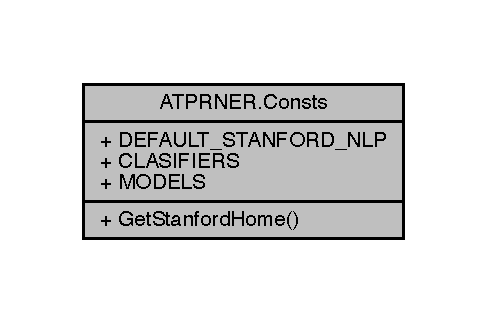
\includegraphics[width=234pt]{d8/dc9/class_a_t_p_r_n_e_r_1_1_consts__coll__graph}
\end{center}
\end{figure}
\subsection*{Static Public Member Functions}
\begin{DoxyCompactItemize}
\item 
static string \hyperlink{class_a_t_p_r_n_e_r_1_1_consts_ad399f9a954d0d35c77fdc899f1c47255}{Get\+Stanford\+Home} ()
\begin{DoxyCompactList}\small\item\em Gets the home for the stanford jars. \end{DoxyCompactList}\end{DoxyCompactItemize}
\subsection*{Static Public Attributes}
\begin{DoxyCompactItemize}
\item 
static string \hyperlink{class_a_t_p_r_n_e_r_1_1_consts_a5552c464404a06a1cb4903e9e8a6fd19}{D\+E\+F\+A\+U\+L\+T\+\_\+\+S\+T\+A\+N\+F\+O\+R\+D\+\_\+\+N\+LP} = Environment.\+Get\+Environment\+Variable(\char`\"{}H\+O\+ME\char`\"{}) + \char`\"{}/Hackaton/Stanford/\char`\"{}
\begin{DoxyCompactList}\small\item\em The default stanford nlp directory. \end{DoxyCompactList}\item 
static string \hyperlink{class_a_t_p_r_n_e_r_1_1_consts_a2c6cdaf05bd4a84d141e3cdd19205f4d}{C\+L\+A\+S\+I\+F\+I\+E\+RS} = @\char`\"{}/stanford-\/ner-\/2015-\/12-\/09/classifiers/\char`\"{}
\begin{DoxyCompactList}\small\item\em The clasifiers directory. \end{DoxyCompactList}\item 
static string \hyperlink{class_a_t_p_r_n_e_r_1_1_consts_a2e80ccd5f9a0b20cf5ce31386604a3b2}{M\+O\+D\+E\+LS} = @\char`\"{}/spanish.\+ancora.\+distsim.\+s512.\+crf.\+ser.\+gz\char`\"{}
\begin{DoxyCompactList}\small\item\em The spanish models. \end{DoxyCompactList}\end{DoxyCompactItemize}


\subsection{Member Function Documentation}
\hypertarget{class_a_t_p_r_n_e_r_1_1_consts_ad399f9a954d0d35c77fdc899f1c47255}{}\label{class_a_t_p_r_n_e_r_1_1_consts_ad399f9a954d0d35c77fdc899f1c47255} 
\index{A\+T\+P\+R\+N\+E\+R\+::\+Consts@{A\+T\+P\+R\+N\+E\+R\+::\+Consts}!Get\+Stanford\+Home@{Get\+Stanford\+Home}}
\index{Get\+Stanford\+Home@{Get\+Stanford\+Home}!A\+T\+P\+R\+N\+E\+R\+::\+Consts@{A\+T\+P\+R\+N\+E\+R\+::\+Consts}}
\subsubsection{\texorpdfstring{Get\+Stanford\+Home()}{GetStanfordHome()}}
{\footnotesize\ttfamily static string A\+T\+P\+R\+N\+E\+R.\+Consts.\+Get\+Stanford\+Home (\begin{DoxyParamCaption}{ }\end{DoxyParamCaption})\hspace{0.3cm}{\ttfamily [inline]}, {\ttfamily [static]}}



Gets the home for the stanford jars. 

\begin{DoxyReturn}{Returns}
The stanford home path
\end{DoxyReturn}
Here is the caller graph for this function\+:
\nopagebreak
\begin{figure}[H]
\begin{center}
\leavevmode
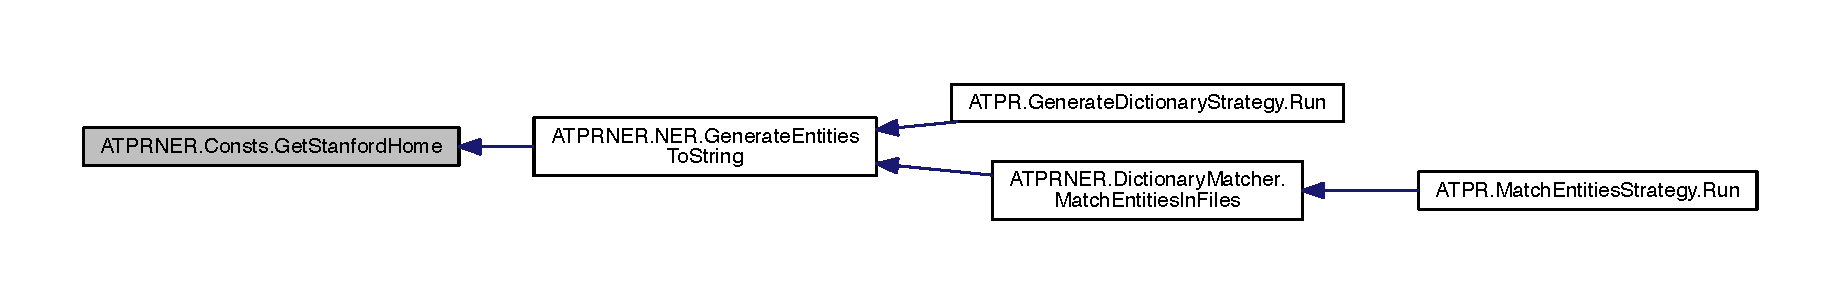
\includegraphics[width=350pt]{d4/d4f/class_a_t_p_r_n_e_r_1_1_consts_ad399f9a954d0d35c77fdc899f1c47255_icgraph}
\end{center}
\end{figure}


\subsection{Member Data Documentation}
\hypertarget{class_a_t_p_r_n_e_r_1_1_consts_a2c6cdaf05bd4a84d141e3cdd19205f4d}{}\label{class_a_t_p_r_n_e_r_1_1_consts_a2c6cdaf05bd4a84d141e3cdd19205f4d} 
\index{A\+T\+P\+R\+N\+E\+R\+::\+Consts@{A\+T\+P\+R\+N\+E\+R\+::\+Consts}!C\+L\+A\+S\+I\+F\+I\+E\+RS@{C\+L\+A\+S\+I\+F\+I\+E\+RS}}
\index{C\+L\+A\+S\+I\+F\+I\+E\+RS@{C\+L\+A\+S\+I\+F\+I\+E\+RS}!A\+T\+P\+R\+N\+E\+R\+::\+Consts@{A\+T\+P\+R\+N\+E\+R\+::\+Consts}}
\subsubsection{\texorpdfstring{C\+L\+A\+S\+I\+F\+I\+E\+RS}{CLASIFIERS}}
{\footnotesize\ttfamily string A\+T\+P\+R\+N\+E\+R.\+Consts.\+C\+L\+A\+S\+I\+F\+I\+E\+RS = @\char`\"{}/stanford-\/ner-\/2015-\/12-\/09/classifiers/\char`\"{}\hspace{0.3cm}{\ttfamily [static]}}



The clasifiers directory. 

\hypertarget{class_a_t_p_r_n_e_r_1_1_consts_a5552c464404a06a1cb4903e9e8a6fd19}{}\label{class_a_t_p_r_n_e_r_1_1_consts_a5552c464404a06a1cb4903e9e8a6fd19} 
\index{A\+T\+P\+R\+N\+E\+R\+::\+Consts@{A\+T\+P\+R\+N\+E\+R\+::\+Consts}!D\+E\+F\+A\+U\+L\+T\+\_\+\+S\+T\+A\+N\+F\+O\+R\+D\+\_\+\+N\+LP@{D\+E\+F\+A\+U\+L\+T\+\_\+\+S\+T\+A\+N\+F\+O\+R\+D\+\_\+\+N\+LP}}
\index{D\+E\+F\+A\+U\+L\+T\+\_\+\+S\+T\+A\+N\+F\+O\+R\+D\+\_\+\+N\+LP@{D\+E\+F\+A\+U\+L\+T\+\_\+\+S\+T\+A\+N\+F\+O\+R\+D\+\_\+\+N\+LP}!A\+T\+P\+R\+N\+E\+R\+::\+Consts@{A\+T\+P\+R\+N\+E\+R\+::\+Consts}}
\subsubsection{\texorpdfstring{D\+E\+F\+A\+U\+L\+T\+\_\+\+S\+T\+A\+N\+F\+O\+R\+D\+\_\+\+N\+LP}{DEFAULT\_STANFORD\_NLP}}
{\footnotesize\ttfamily string A\+T\+P\+R\+N\+E\+R.\+Consts.\+D\+E\+F\+A\+U\+L\+T\+\_\+\+S\+T\+A\+N\+F\+O\+R\+D\+\_\+\+N\+LP = Environment.\+Get\+Environment\+Variable(\char`\"{}H\+O\+ME\char`\"{}) + \char`\"{}/Hackaton/Stanford/\char`\"{}\hspace{0.3cm}{\ttfamily [static]}}



The default stanford nlp directory. 

\hypertarget{class_a_t_p_r_n_e_r_1_1_consts_a2e80ccd5f9a0b20cf5ce31386604a3b2}{}\label{class_a_t_p_r_n_e_r_1_1_consts_a2e80ccd5f9a0b20cf5ce31386604a3b2} 
\index{A\+T\+P\+R\+N\+E\+R\+::\+Consts@{A\+T\+P\+R\+N\+E\+R\+::\+Consts}!M\+O\+D\+E\+LS@{M\+O\+D\+E\+LS}}
\index{M\+O\+D\+E\+LS@{M\+O\+D\+E\+LS}!A\+T\+P\+R\+N\+E\+R\+::\+Consts@{A\+T\+P\+R\+N\+E\+R\+::\+Consts}}
\subsubsection{\texorpdfstring{M\+O\+D\+E\+LS}{MODELS}}
{\footnotesize\ttfamily string A\+T\+P\+R\+N\+E\+R.\+Consts.\+M\+O\+D\+E\+LS = @\char`\"{}/spanish.\+ancora.\+distsim.\+s512.\+crf.\+ser.\+gz\char`\"{}\hspace{0.3cm}{\ttfamily [static]}}



The spanish models. 



The documentation for this class was generated from the following file\+:\begin{DoxyCompactItemize}
\item 
A\+T\+P\+R\+N\+E\+R/Consts.\+cs\end{DoxyCompactItemize}

\hypertarget{class_a_t_p_r_parser_1_1_consts}{}\section{A\+T\+P\+R\+Parser.\+Consts Class Reference}
\label{class_a_t_p_r_parser_1_1_consts}\index{A\+T\+P\+R\+Parser.\+Consts@{A\+T\+P\+R\+Parser.\+Consts}}


Collaboration diagram for A\+T\+P\+R\+Parser.\+Consts\+:
\nopagebreak
\begin{figure}[H]
\begin{center}
\leavevmode
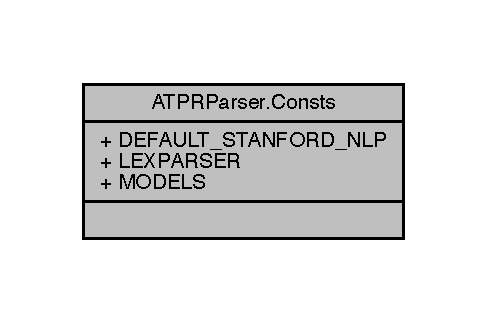
\includegraphics[width=234pt]{db/d18/class_a_t_p_r_parser_1_1_consts__coll__graph}
\end{center}
\end{figure}
\subsection*{Static Public Attributes}
\begin{DoxyCompactItemize}
\item 
static string \hyperlink{class_a_t_p_r_parser_1_1_consts_a2a255a7847f7123ddac4b35f829f8ad5}{D\+E\+F\+A\+U\+L\+T\+\_\+\+S\+T\+A\+N\+F\+O\+R\+D\+\_\+\+N\+LP} = Environment.\+Get\+Environment\+Variable(\char`\"{}H\+O\+ME\char`\"{}) + \char`\"{}/Hackaton/Stanford/\char`\"{}
\begin{DoxyCompactList}\small\item\em The default stanford nlp directory. \end{DoxyCompactList}\item 
static string \hyperlink{class_a_t_p_r_parser_1_1_consts_ab61b6ffd61033d649b5eed2c68fd253c}{L\+E\+X\+P\+A\+R\+S\+ER} = @\char`\"{}/lexparser/spanish\+P\+C\+F\+G.\+ser.\+gz\char`\"{}
\begin{DoxyCompactList}\small\item\em The L\+E\+X\+P\+A\+R\+S\+ER directory. \end{DoxyCompactList}\item 
static string \hyperlink{class_a_t_p_r_parser_1_1_consts_af9e34e76e089c4884245fd4a79c09e2c}{M\+O\+D\+E\+LS} = @\char`\"{}/edu/stanford/nlp/models\char`\"{}
\begin{DoxyCompactList}\small\item\em The spanish models. \end{DoxyCompactList}\end{DoxyCompactItemize}


\subsection{Member Data Documentation}
\hypertarget{class_a_t_p_r_parser_1_1_consts_a2a255a7847f7123ddac4b35f829f8ad5}{}\label{class_a_t_p_r_parser_1_1_consts_a2a255a7847f7123ddac4b35f829f8ad5} 
\index{A\+T\+P\+R\+Parser\+::\+Consts@{A\+T\+P\+R\+Parser\+::\+Consts}!D\+E\+F\+A\+U\+L\+T\+\_\+\+S\+T\+A\+N\+F\+O\+R\+D\+\_\+\+N\+LP@{D\+E\+F\+A\+U\+L\+T\+\_\+\+S\+T\+A\+N\+F\+O\+R\+D\+\_\+\+N\+LP}}
\index{D\+E\+F\+A\+U\+L\+T\+\_\+\+S\+T\+A\+N\+F\+O\+R\+D\+\_\+\+N\+LP@{D\+E\+F\+A\+U\+L\+T\+\_\+\+S\+T\+A\+N\+F\+O\+R\+D\+\_\+\+N\+LP}!A\+T\+P\+R\+Parser\+::\+Consts@{A\+T\+P\+R\+Parser\+::\+Consts}}
\subsubsection{\texorpdfstring{D\+E\+F\+A\+U\+L\+T\+\_\+\+S\+T\+A\+N\+F\+O\+R\+D\+\_\+\+N\+LP}{DEFAULT\_STANFORD\_NLP}}
{\footnotesize\ttfamily string A\+T\+P\+R\+Parser.\+Consts.\+D\+E\+F\+A\+U\+L\+T\+\_\+\+S\+T\+A\+N\+F\+O\+R\+D\+\_\+\+N\+LP = Environment.\+Get\+Environment\+Variable(\char`\"{}H\+O\+ME\char`\"{}) + \char`\"{}/Hackaton/Stanford/\char`\"{}\hspace{0.3cm}{\ttfamily [static]}}



The default stanford nlp directory. 

\hypertarget{class_a_t_p_r_parser_1_1_consts_ab61b6ffd61033d649b5eed2c68fd253c}{}\label{class_a_t_p_r_parser_1_1_consts_ab61b6ffd61033d649b5eed2c68fd253c} 
\index{A\+T\+P\+R\+Parser\+::\+Consts@{A\+T\+P\+R\+Parser\+::\+Consts}!L\+E\+X\+P\+A\+R\+S\+ER@{L\+E\+X\+P\+A\+R\+S\+ER}}
\index{L\+E\+X\+P\+A\+R\+S\+ER@{L\+E\+X\+P\+A\+R\+S\+ER}!A\+T\+P\+R\+Parser\+::\+Consts@{A\+T\+P\+R\+Parser\+::\+Consts}}
\subsubsection{\texorpdfstring{L\+E\+X\+P\+A\+R\+S\+ER}{LEXPARSER}}
{\footnotesize\ttfamily string A\+T\+P\+R\+Parser.\+Consts.\+L\+E\+X\+P\+A\+R\+S\+ER = @\char`\"{}/lexparser/spanish\+P\+C\+F\+G.\+ser.\+gz\char`\"{}\hspace{0.3cm}{\ttfamily [static]}}



The L\+E\+X\+P\+A\+R\+S\+ER directory. 

\hypertarget{class_a_t_p_r_parser_1_1_consts_af9e34e76e089c4884245fd4a79c09e2c}{}\label{class_a_t_p_r_parser_1_1_consts_af9e34e76e089c4884245fd4a79c09e2c} 
\index{A\+T\+P\+R\+Parser\+::\+Consts@{A\+T\+P\+R\+Parser\+::\+Consts}!M\+O\+D\+E\+LS@{M\+O\+D\+E\+LS}}
\index{M\+O\+D\+E\+LS@{M\+O\+D\+E\+LS}!A\+T\+P\+R\+Parser\+::\+Consts@{A\+T\+P\+R\+Parser\+::\+Consts}}
\subsubsection{\texorpdfstring{M\+O\+D\+E\+LS}{MODELS}}
{\footnotesize\ttfamily string A\+T\+P\+R\+Parser.\+Consts.\+M\+O\+D\+E\+LS = @\char`\"{}/edu/stanford/nlp/models\char`\"{}\hspace{0.3cm}{\ttfamily [static]}}



The spanish models. 



The documentation for this class was generated from the following file\+:\begin{DoxyCompactItemize}
\item 
A\+T\+P\+R\+P\+A\+R\+S\+E\+R/Consts.\+cs\end{DoxyCompactItemize}

\hypertarget{class_a_t_p_r_n_e_r_1_1_c_s_v_utils}{}\section{A\+T\+P\+R\+N\+E\+R.\+C\+S\+V\+Utils Class Reference}
\label{class_a_t_p_r_n_e_r_1_1_c_s_v_utils}\index{A\+T\+P\+R\+N\+E\+R.\+C\+S\+V\+Utils@{A\+T\+P\+R\+N\+E\+R.\+C\+S\+V\+Utils}}
\subsection*{Static Public Member Functions}
\begin{DoxyCompactItemize}
\item 
static string \hyperlink{class_a_t_p_r_n_e_r_1_1_c_s_v_utils_adfa299109e3212e72e6468644b0bdd0c}{Entities\+To\+Csv} (string entities\+Xml)
\begin{DoxyCompactList}\small\item\em From a \hyperlink{class_a_t_p_r_n_e_r_1_1_n_e_r}{N\+ER} xml entities returns a C\+SV with the interesting entities \end{DoxyCompactList}\item 
static string \hyperlink{class_a_t_p_r_n_e_r_1_1_c_s_v_utils_ab236c362e83053e0e7165aa2e45849c4}{Remove\+Duplicates} (string csv)
\begin{DoxyCompactList}\small\item\em Removes the duplicates from a C\+SV. \end{DoxyCompactList}\end{DoxyCompactItemize}


\subsection{Member Function Documentation}
\hypertarget{class_a_t_p_r_n_e_r_1_1_c_s_v_utils_adfa299109e3212e72e6468644b0bdd0c}{}\label{class_a_t_p_r_n_e_r_1_1_c_s_v_utils_adfa299109e3212e72e6468644b0bdd0c} 
\index{A\+T\+P\+R\+N\+E\+R\+::\+C\+S\+V\+Utils@{A\+T\+P\+R\+N\+E\+R\+::\+C\+S\+V\+Utils}!Entities\+To\+Csv@{Entities\+To\+Csv}}
\index{Entities\+To\+Csv@{Entities\+To\+Csv}!A\+T\+P\+R\+N\+E\+R\+::\+C\+S\+V\+Utils@{A\+T\+P\+R\+N\+E\+R\+::\+C\+S\+V\+Utils}}
\subsubsection{\texorpdfstring{Entities\+To\+Csv()}{EntitiesToCsv()}}
{\footnotesize\ttfamily static string A\+T\+P\+R\+N\+E\+R.\+C\+S\+V\+Utils.\+Entities\+To\+Csv (\begin{DoxyParamCaption}\item[{string}]{entities\+Xml }\end{DoxyParamCaption})\hspace{0.3cm}{\ttfamily [inline]}, {\ttfamily [static]}}



From a \hyperlink{class_a_t_p_r_n_e_r_1_1_n_e_r}{N\+ER} xml entities returns a C\+SV with the interesting entities 

\begin{DoxyReturn}{Returns}
The entities in C\+SV.
\end{DoxyReturn}

\begin{DoxyParams}{Parameters}
{\em entities\+Xml} & Entities xml.\\
\hline
\end{DoxyParams}
\hypertarget{class_a_t_p_r_n_e_r_1_1_c_s_v_utils_ab236c362e83053e0e7165aa2e45849c4}{}\label{class_a_t_p_r_n_e_r_1_1_c_s_v_utils_ab236c362e83053e0e7165aa2e45849c4} 
\index{A\+T\+P\+R\+N\+E\+R\+::\+C\+S\+V\+Utils@{A\+T\+P\+R\+N\+E\+R\+::\+C\+S\+V\+Utils}!Remove\+Duplicates@{Remove\+Duplicates}}
\index{Remove\+Duplicates@{Remove\+Duplicates}!A\+T\+P\+R\+N\+E\+R\+::\+C\+S\+V\+Utils@{A\+T\+P\+R\+N\+E\+R\+::\+C\+S\+V\+Utils}}
\subsubsection{\texorpdfstring{Remove\+Duplicates()}{RemoveDuplicates()}}
{\footnotesize\ttfamily static string A\+T\+P\+R\+N\+E\+R.\+C\+S\+V\+Utils.\+Remove\+Duplicates (\begin{DoxyParamCaption}\item[{string}]{csv }\end{DoxyParamCaption})\hspace{0.3cm}{\ttfamily [inline]}, {\ttfamily [static]}}



Removes the duplicates from a C\+SV. 

\begin{DoxyReturn}{Returns}
The duplicates.
\end{DoxyReturn}

\begin{DoxyParams}{Parameters}
{\em csv} & Csv.\\
\hline
\end{DoxyParams}


The documentation for this class was generated from the following file\+:\begin{DoxyCompactItemize}
\item 
A\+T\+P\+R\+N\+E\+R/C\+S\+V\+Utils.\+cs\end{DoxyCompactItemize}

\hypertarget{class_a_t_p_r_n_e_r_1_1_dictionary_matcher}{}\section{A\+T\+P\+R\+N\+E\+R.\+Dictionary\+Matcher Class Reference}
\label{class_a_t_p_r_n_e_r_1_1_dictionary_matcher}\index{A\+T\+P\+R\+N\+E\+R.\+Dictionary\+Matcher@{A\+T\+P\+R\+N\+E\+R.\+Dictionary\+Matcher}}


Collaboration diagram for A\+T\+P\+R\+N\+E\+R.\+Dictionary\+Matcher\+:
\nopagebreak
\begin{figure}[H]
\begin{center}
\leavevmode
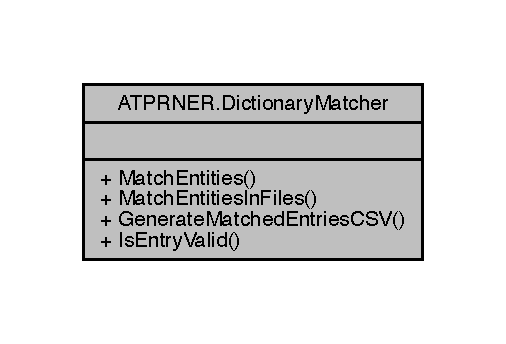
\includegraphics[width=226pt]{db/d42/class_a_t_p_r_n_e_r_1_1_dictionary_matcher__coll__graph}
\end{center}
\end{figure}
\subsection*{Static Public Member Functions}
\begin{DoxyCompactItemize}
\item 
static Dictionary$<$ string, \hyperlink{class_a_t_p_r_n_e_r_1_1_matched_entity}{Matched\+Entity} $>$ \hyperlink{class_a_t_p_r_n_e_r_1_1_dictionary_matcher_aa6fdeaf3a88c14b5ed8e4f452d1c3c17}{Match\+Entities} (List$<$ string\mbox{[}$\,$\mbox{]}$>$ text\+Entities, List$<$ string $>$ dict\+Entities)
\begin{DoxyCompactList}\small\item\em Matchs the text entities with the dictionary entities. \end{DoxyCompactList}\item 
static void \hyperlink{class_a_t_p_r_n_e_r_1_1_dictionary_matcher_a6fc36cbd0e0df420c2aaafa389ae7b61}{Match\+Entities\+In\+Files} (string input\+Path, string dic\+Path, Text\+Writer output, char sep)
\begin{DoxyCompactList}\small\item\em Writes to the output stream a csv with the match results against the dictionary \end{DoxyCompactList}\end{DoxyCompactItemize}


\subsection{Member Function Documentation}
\hypertarget{class_a_t_p_r_n_e_r_1_1_dictionary_matcher_aa6fdeaf3a88c14b5ed8e4f452d1c3c17}{}\label{class_a_t_p_r_n_e_r_1_1_dictionary_matcher_aa6fdeaf3a88c14b5ed8e4f452d1c3c17} 
\index{A\+T\+P\+R\+N\+E\+R\+::\+Dictionary\+Matcher@{A\+T\+P\+R\+N\+E\+R\+::\+Dictionary\+Matcher}!Match\+Entities@{Match\+Entities}}
\index{Match\+Entities@{Match\+Entities}!A\+T\+P\+R\+N\+E\+R\+::\+Dictionary\+Matcher@{A\+T\+P\+R\+N\+E\+R\+::\+Dictionary\+Matcher}}
\subsubsection{\texorpdfstring{Match\+Entities()}{MatchEntities()}}
{\footnotesize\ttfamily static Dictionary$<$string, \hyperlink{class_a_t_p_r_n_e_r_1_1_matched_entity}{Matched\+Entity}$>$ A\+T\+P\+R\+N\+E\+R.\+Dictionary\+Matcher.\+Match\+Entities (\begin{DoxyParamCaption}\item[{List$<$ string\mbox{[}$\,$\mbox{]}$>$}]{text\+Entities,  }\item[{List$<$ string $>$}]{dict\+Entities }\end{DoxyParamCaption})\hspace{0.3cm}{\ttfamily [inline]}, {\ttfamily [static]}}



Matchs the text entities with the dictionary entities. 

\begin{DoxyReturn}{Returns}
The entities.
\end{DoxyReturn}

\begin{DoxyParams}{Parameters}
{\em text\+Entities} & Text entities.\\
\hline
{\em dict\+Entities} & Dict entities.\\
\hline
\end{DoxyParams}
Here is the caller graph for this function\+:
\nopagebreak
\begin{figure}[H]
\begin{center}
\leavevmode
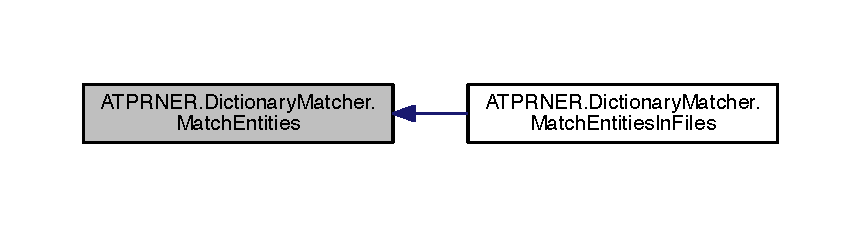
\includegraphics[width=350pt]{d0/d6a/class_a_t_p_r_n_e_r_1_1_dictionary_matcher_aa6fdeaf3a88c14b5ed8e4f452d1c3c17_icgraph}
\end{center}
\end{figure}
\hypertarget{class_a_t_p_r_n_e_r_1_1_dictionary_matcher_a6fc36cbd0e0df420c2aaafa389ae7b61}{}\label{class_a_t_p_r_n_e_r_1_1_dictionary_matcher_a6fc36cbd0e0df420c2aaafa389ae7b61} 
\index{A\+T\+P\+R\+N\+E\+R\+::\+Dictionary\+Matcher@{A\+T\+P\+R\+N\+E\+R\+::\+Dictionary\+Matcher}!Match\+Entities\+In\+Files@{Match\+Entities\+In\+Files}}
\index{Match\+Entities\+In\+Files@{Match\+Entities\+In\+Files}!A\+T\+P\+R\+N\+E\+R\+::\+Dictionary\+Matcher@{A\+T\+P\+R\+N\+E\+R\+::\+Dictionary\+Matcher}}
\subsubsection{\texorpdfstring{Match\+Entities\+In\+Files()}{MatchEntitiesInFiles()}}
{\footnotesize\ttfamily static void A\+T\+P\+R\+N\+E\+R.\+Dictionary\+Matcher.\+Match\+Entities\+In\+Files (\begin{DoxyParamCaption}\item[{string}]{input\+Path,  }\item[{string}]{dic\+Path,  }\item[{Text\+Writer}]{output,  }\item[{char}]{sep }\end{DoxyParamCaption})\hspace{0.3cm}{\ttfamily [inline]}, {\ttfamily [static]}}



Writes to the output stream a csv with the match results against the dictionary 


\begin{DoxyParams}{Parameters}
{\em input\+Path} & Files path.\\
\hline
{\em dic\+Path} & Dictionary path.\\
\hline
{\em output} & Output stream.\\
\hline
\end{DoxyParams}
Here is the call graph for this function\+:
\nopagebreak
\begin{figure}[H]
\begin{center}
\leavevmode
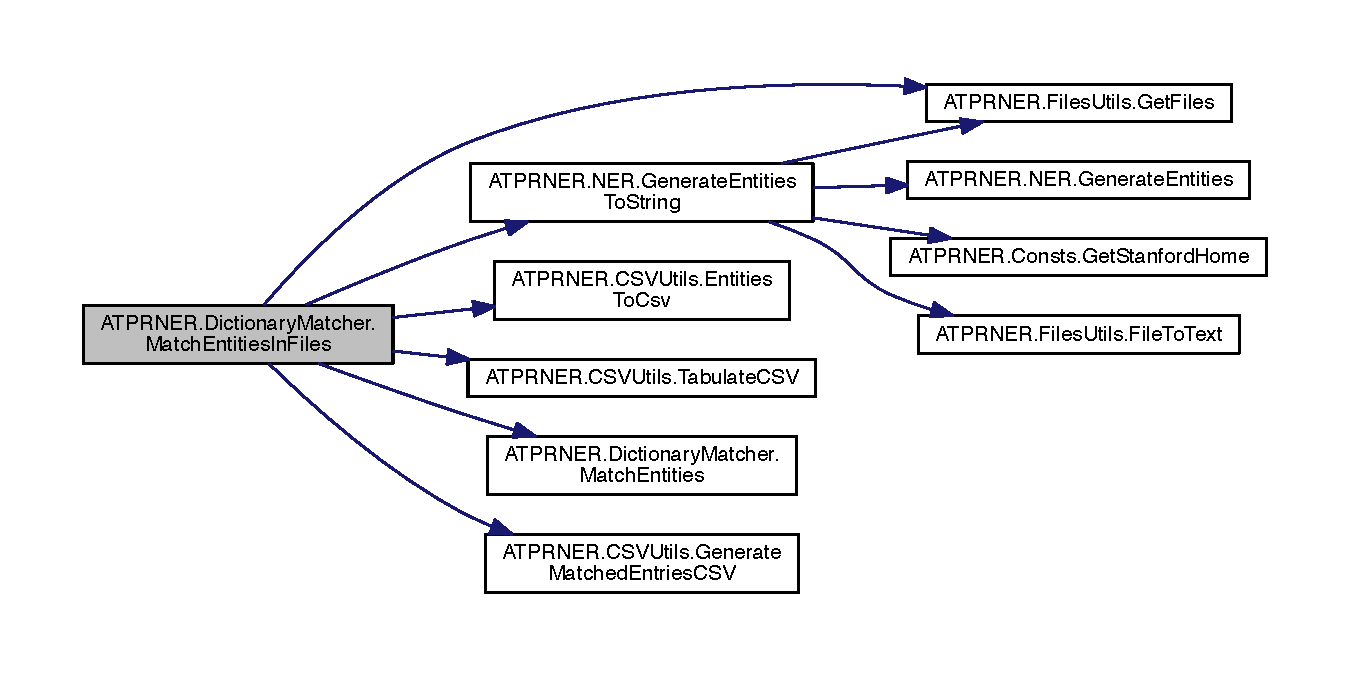
\includegraphics[width=350pt]{d0/d6a/class_a_t_p_r_n_e_r_1_1_dictionary_matcher_a6fc36cbd0e0df420c2aaafa389ae7b61_cgraph}
\end{center}
\end{figure}
Here is the caller graph for this function\+:
\nopagebreak
\begin{figure}[H]
\begin{center}
\leavevmode
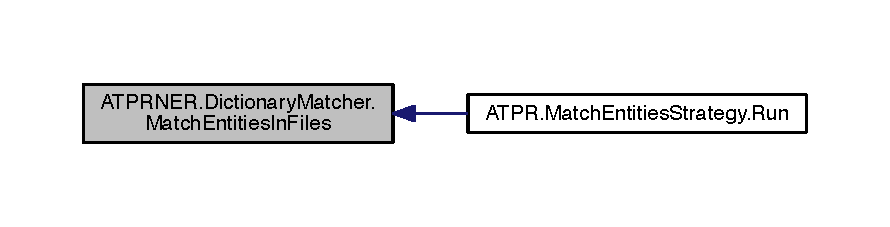
\includegraphics[width=350pt]{d0/d6a/class_a_t_p_r_n_e_r_1_1_dictionary_matcher_a6fc36cbd0e0df420c2aaafa389ae7b61_icgraph}
\end{center}
\end{figure}


The documentation for this class was generated from the following file\+:\begin{DoxyCompactItemize}
\item 
A\+T\+P\+R\+N\+E\+R/Dictionary\+Matcher.\+cs\end{DoxyCompactItemize}

\hypertarget{interface_a_t_p_r_1_1_exec_strategy}{}\section{A\+T\+P\+R.\+Exec\+Strategy Interface Reference}
\label{interface_a_t_p_r_1_1_exec_strategy}\index{A\+T\+P\+R.\+Exec\+Strategy@{A\+T\+P\+R.\+Exec\+Strategy}}


Base interface for strategy classes  




Inheritance diagram for A\+T\+P\+R.\+Exec\+Strategy\+:
\nopagebreak
\begin{figure}[H]
\begin{center}
\leavevmode
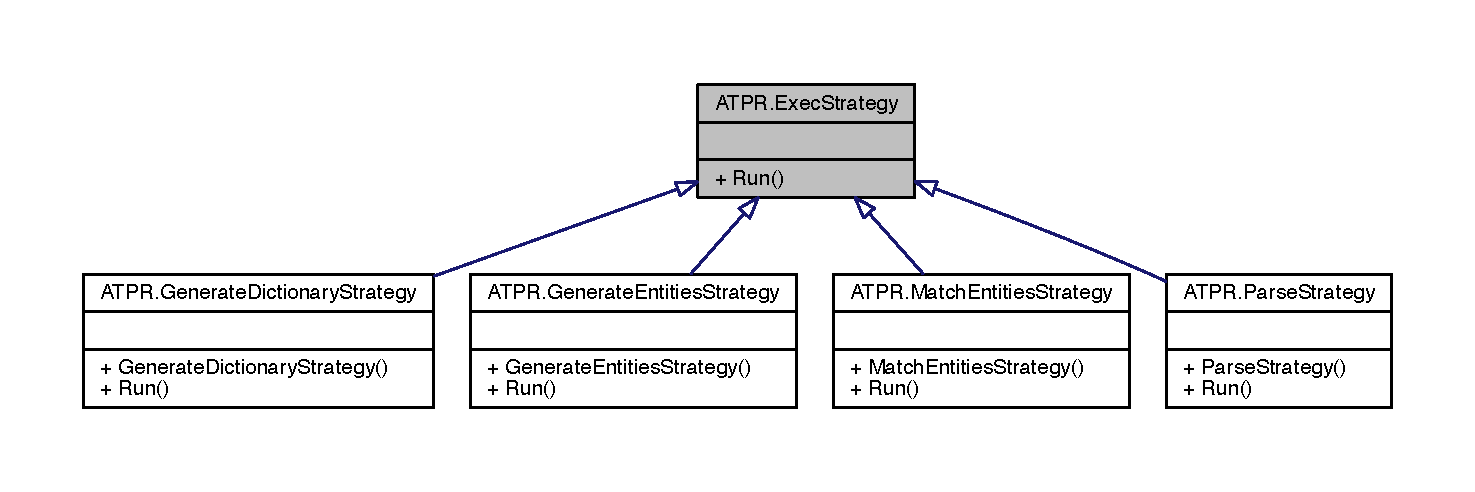
\includegraphics[width=221pt]{d2/d3b/interface_a_t_p_r_1_1_exec_strategy__inherit__graph}
\end{center}
\end{figure}


Collaboration diagram for A\+T\+P\+R.\+Exec\+Strategy\+:
\nopagebreak
\begin{figure}[H]
\begin{center}
\leavevmode
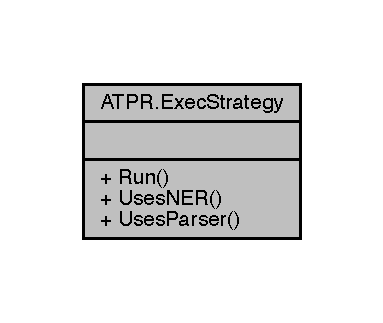
\includegraphics[width=184pt]{d9/db3/interface_a_t_p_r_1_1_exec_strategy__coll__graph}
\end{center}
\end{figure}
\subsection*{Public Member Functions}
\begin{DoxyCompactItemize}
\item 
\hypertarget{interface_a_t_p_r_1_1_exec_strategy_adcd52fae2702ce31b645ec8d149c0e51}{}\label{interface_a_t_p_r_1_1_exec_strategy_adcd52fae2702ce31b645ec8d149c0e51} 
void {\bfseries Run} ()
\item 
\hypertarget{interface_a_t_p_r_1_1_exec_strategy_acd32c810cb2247e7b058520cce7ed3cb}{}\label{interface_a_t_p_r_1_1_exec_strategy_acd32c810cb2247e7b058520cce7ed3cb} 
bool {\bfseries Uses\+N\+ER} ()
\item 
\hypertarget{interface_a_t_p_r_1_1_exec_strategy_a04e0c2d18b63468c4255c08182620726}{}\label{interface_a_t_p_r_1_1_exec_strategy_a04e0c2d18b63468c4255c08182620726} 
bool {\bfseries Uses\+Parser} ()
\end{DoxyCompactItemize}


\subsection{Detailed Description}
Base interface for strategy classes 



The documentation for this interface was generated from the following file\+:\begin{DoxyCompactItemize}
\item 
A\+T\+P\+R/Exec\+Strategy.\+cs\end{DoxyCompactItemize}

\hypertarget{class_a_t_p_r_n_e_r_1_1_files_utils}{}\section{A\+T\+P\+R\+N\+E\+R.\+Files\+Utils Class Reference}
\label{class_a_t_p_r_n_e_r_1_1_files_utils}\index{A\+T\+P\+R\+N\+E\+R.\+Files\+Utils@{A\+T\+P\+R\+N\+E\+R.\+Files\+Utils}}


Collaboration diagram for A\+T\+P\+R\+N\+E\+R.\+Files\+Utils\+:
\nopagebreak
\begin{figure}[H]
\begin{center}
\leavevmode
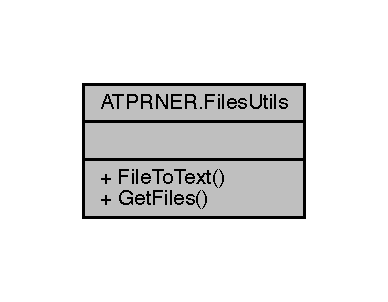
\includegraphics[width=186pt]{d5/dc5/class_a_t_p_r_n_e_r_1_1_files_utils__coll__graph}
\end{center}
\end{figure}
\subsection*{Static Public Member Functions}
\begin{DoxyCompactItemize}
\item 
static string \hyperlink{class_a_t_p_r_n_e_r_1_1_files_utils_adaf763c34895368bcfe1254086d87f99}{File\+To\+Text} (string file\+Path)
\begin{DoxyCompactList}\small\item\em Extrat the text from a file, using Toxy for binary files. \end{DoxyCompactList}\item 
static string \mbox{[}$\,$\mbox{]} \hyperlink{class_a_t_p_r_n_e_r_1_1_files_utils_aa9ee9ca4b22ddc16322bff7ea1d979bb}{Get\+Files} (string input\+Path)
\begin{DoxyCompactList}\small\item\em Returns an array of files to be parsed \end{DoxyCompactList}\end{DoxyCompactItemize}


\subsection{Member Function Documentation}
\hypertarget{class_a_t_p_r_n_e_r_1_1_files_utils_adaf763c34895368bcfe1254086d87f99}{}\label{class_a_t_p_r_n_e_r_1_1_files_utils_adaf763c34895368bcfe1254086d87f99} 
\index{A\+T\+P\+R\+N\+E\+R\+::\+Files\+Utils@{A\+T\+P\+R\+N\+E\+R\+::\+Files\+Utils}!File\+To\+Text@{File\+To\+Text}}
\index{File\+To\+Text@{File\+To\+Text}!A\+T\+P\+R\+N\+E\+R\+::\+Files\+Utils@{A\+T\+P\+R\+N\+E\+R\+::\+Files\+Utils}}
\subsubsection{\texorpdfstring{File\+To\+Text()}{FileToText()}}
{\footnotesize\ttfamily static string A\+T\+P\+R\+N\+E\+R.\+Files\+Utils.\+File\+To\+Text (\begin{DoxyParamCaption}\item[{string}]{file\+Path }\end{DoxyParamCaption})\hspace{0.3cm}{\ttfamily [inline]}, {\ttfamily [static]}}



Extrat the text from a file, using Toxy for binary files. 

\begin{DoxyReturn}{Returns}
The plain text of the document
\end{DoxyReturn}

\begin{DoxyParams}{Parameters}
{\em file\+Path} & File path.\\
\hline
\end{DoxyParams}
Here is the caller graph for this function\+:
\nopagebreak
\begin{figure}[H]
\begin{center}
\leavevmode
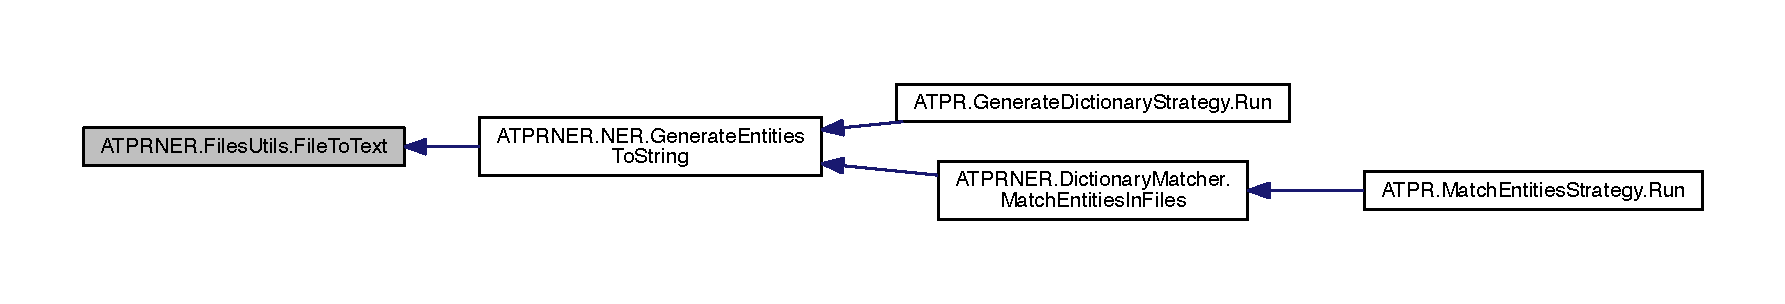
\includegraphics[width=350pt]{d5/de9/class_a_t_p_r_n_e_r_1_1_files_utils_adaf763c34895368bcfe1254086d87f99_icgraph}
\end{center}
\end{figure}
\hypertarget{class_a_t_p_r_n_e_r_1_1_files_utils_aa9ee9ca4b22ddc16322bff7ea1d979bb}{}\label{class_a_t_p_r_n_e_r_1_1_files_utils_aa9ee9ca4b22ddc16322bff7ea1d979bb} 
\index{A\+T\+P\+R\+N\+E\+R\+::\+Files\+Utils@{A\+T\+P\+R\+N\+E\+R\+::\+Files\+Utils}!Get\+Files@{Get\+Files}}
\index{Get\+Files@{Get\+Files}!A\+T\+P\+R\+N\+E\+R\+::\+Files\+Utils@{A\+T\+P\+R\+N\+E\+R\+::\+Files\+Utils}}
\subsubsection{\texorpdfstring{Get\+Files()}{GetFiles()}}
{\footnotesize\ttfamily static string \mbox{[}$\,$\mbox{]} A\+T\+P\+R\+N\+E\+R.\+Files\+Utils.\+Get\+Files (\begin{DoxyParamCaption}\item[{string}]{input\+Path }\end{DoxyParamCaption})\hspace{0.3cm}{\ttfamily [inline]}, {\ttfamily [static]}}



Returns an array of files to be parsed 

\begin{DoxyReturn}{Returns}
A file paths array
\end{DoxyReturn}

\begin{DoxyParams}{Parameters}
{\em input\+Path} & The input path.\\
\hline
\end{DoxyParams}
Here is the caller graph for this function\+:
\nopagebreak
\begin{figure}[H]
\begin{center}
\leavevmode
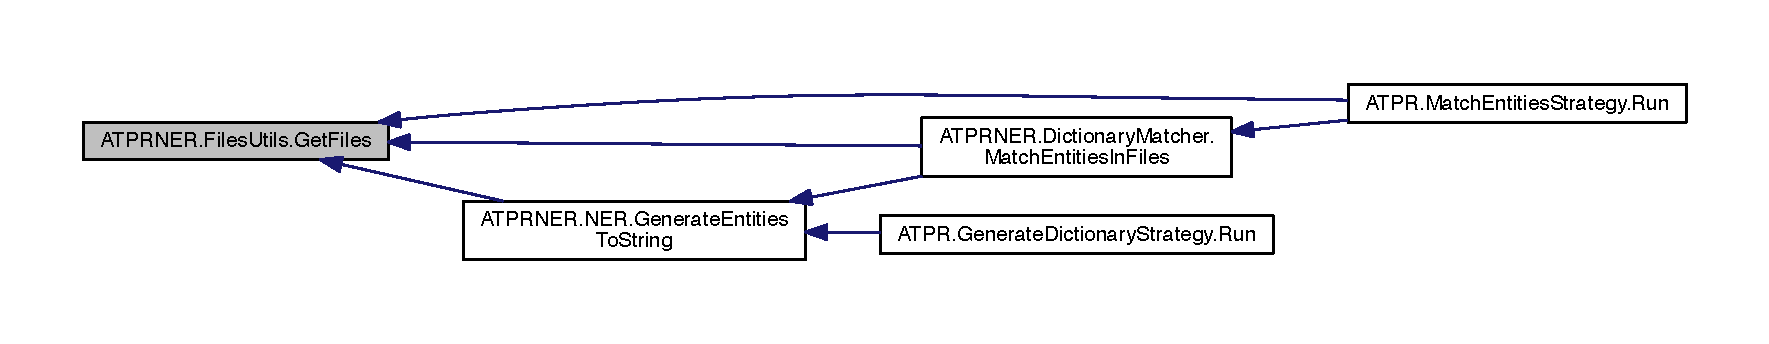
\includegraphics[width=350pt]{d5/de9/class_a_t_p_r_n_e_r_1_1_files_utils_aa9ee9ca4b22ddc16322bff7ea1d979bb_icgraph}
\end{center}
\end{figure}


The documentation for this class was generated from the following file\+:\begin{DoxyCompactItemize}
\item 
A\+T\+P\+R\+N\+E\+R/Files\+Utils.\+cs\end{DoxyCompactItemize}

\hypertarget{class_a_t_p_r_1_1_generate_dictionary_strategy}{}\section{A\+T\+P\+R.\+Generate\+Dictionary\+Strategy Class Reference}
\label{class_a_t_p_r_1_1_generate_dictionary_strategy}\index{A\+T\+P\+R.\+Generate\+Dictionary\+Strategy@{A\+T\+P\+R.\+Generate\+Dictionary\+Strategy}}


Strategy class that generates the dictionary from the N\+ER result.  




Inheritance diagram for A\+T\+P\+R.\+Generate\+Dictionary\+Strategy\+:
\nopagebreak
\begin{figure}[H]
\begin{center}
\leavevmode
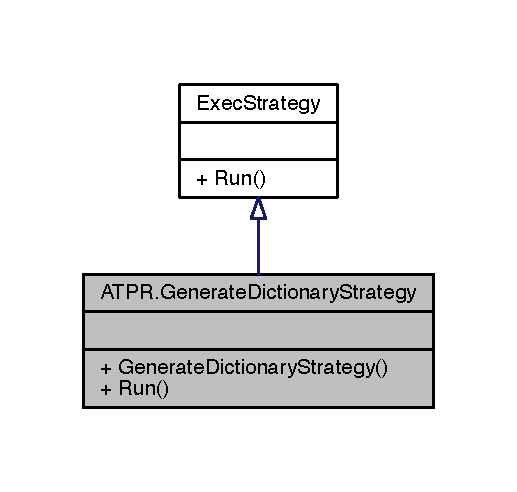
\includegraphics[width=248pt]{d2/d87/class_a_t_p_r_1_1_generate_dictionary_strategy__inherit__graph}
\end{center}
\end{figure}


Collaboration diagram for A\+T\+P\+R.\+Generate\+Dictionary\+Strategy\+:
\nopagebreak
\begin{figure}[H]
\begin{center}
\leavevmode
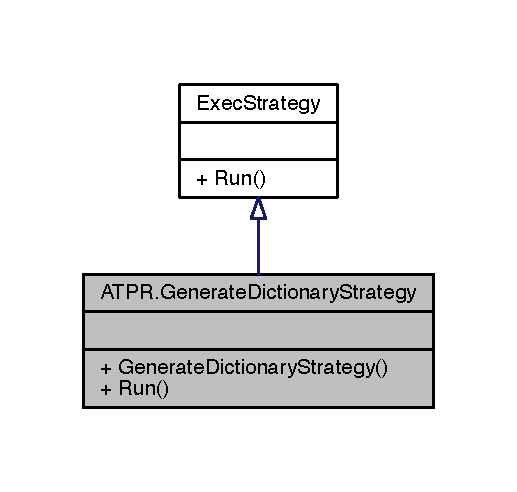
\includegraphics[width=248pt]{de/da4/class_a_t_p_r_1_1_generate_dictionary_strategy__coll__graph}
\end{center}
\end{figure}
\subsection*{Public Member Functions}
\begin{DoxyCompactItemize}
\item 
void \hyperlink{class_a_t_p_r_1_1_generate_dictionary_strategy_acec75993f2d1b9e2899130cd9dff1ffa}{Run} (\hyperlink{class_a_t_p_r_1_1_options}{Options} options)
\begin{DoxyCompactList}\small\item\em Generates the dictionary of entities found. \end{DoxyCompactList}\end{DoxyCompactItemize}


\subsection{Detailed Description}
Strategy class that generates the dictionary from the N\+ER result. 



\subsection{Member Function Documentation}
\hypertarget{class_a_t_p_r_1_1_generate_dictionary_strategy_acec75993f2d1b9e2899130cd9dff1ffa}{}\label{class_a_t_p_r_1_1_generate_dictionary_strategy_acec75993f2d1b9e2899130cd9dff1ffa} 
\index{A\+T\+P\+R\+::\+Generate\+Dictionary\+Strategy@{A\+T\+P\+R\+::\+Generate\+Dictionary\+Strategy}!Run@{Run}}
\index{Run@{Run}!A\+T\+P\+R\+::\+Generate\+Dictionary\+Strategy@{A\+T\+P\+R\+::\+Generate\+Dictionary\+Strategy}}
\subsubsection{\texorpdfstring{Run()}{Run()}}
{\footnotesize\ttfamily void A\+T\+P\+R.\+Generate\+Dictionary\+Strategy.\+Run (\begin{DoxyParamCaption}\item[{\hyperlink{class_a_t_p_r_1_1_options}{Options}}]{options }\end{DoxyParamCaption})\hspace{0.3cm}{\ttfamily [inline]}}



Generates the dictionary of entities found. 


\begin{DoxyParams}{Parameters}
{\em options} & \hyperlink{class_a_t_p_r_1_1_options}{Options}.\\
\hline
\end{DoxyParams}


Implements \hyperlink{interface_a_t_p_r_1_1_exec_strategy}{A\+T\+P\+R.\+Exec\+Strategy}.

Here is the call graph for this function\+:
\nopagebreak
\begin{figure}[H]
\begin{center}
\leavevmode
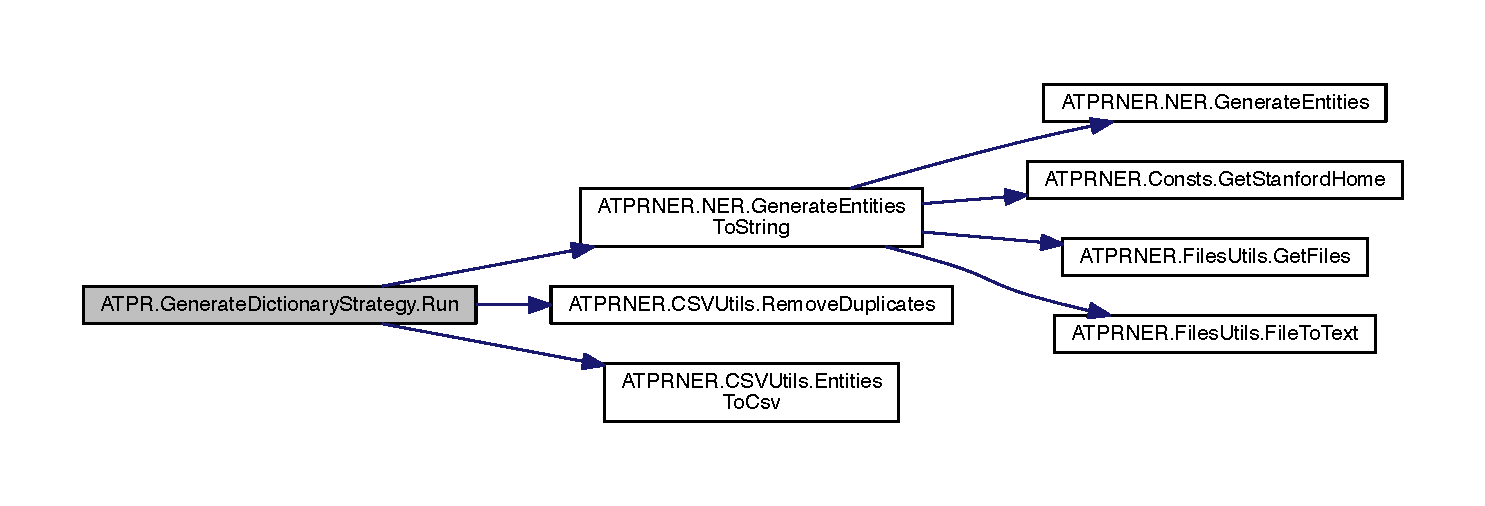
\includegraphics[width=350pt]{d2/d22/class_a_t_p_r_1_1_generate_dictionary_strategy_acec75993f2d1b9e2899130cd9dff1ffa_cgraph}
\end{center}
\end{figure}


The documentation for this class was generated from the following file\+:\begin{DoxyCompactItemize}
\item 
A\+T\+P\+R/Generate\+Dictionary\+Strategy.\+cs\end{DoxyCompactItemize}

\hypertarget{class_a_t_p_r_1_1_generate_entities_strategy}{}\section{A\+T\+P\+R.\+Generate\+Entities\+Strategy Class Reference}
\label{class_a_t_p_r_1_1_generate_entities_strategy}\index{A\+T\+P\+R.\+Generate\+Entities\+Strategy@{A\+T\+P\+R.\+Generate\+Entities\+Strategy}}


s\+Strategy class that check generate entities command arguments and execute generate entities.  




Inheritance diagram for A\+T\+P\+R.\+Generate\+Entities\+Strategy\+:
\nopagebreak
\begin{figure}[H]
\begin{center}
\leavevmode
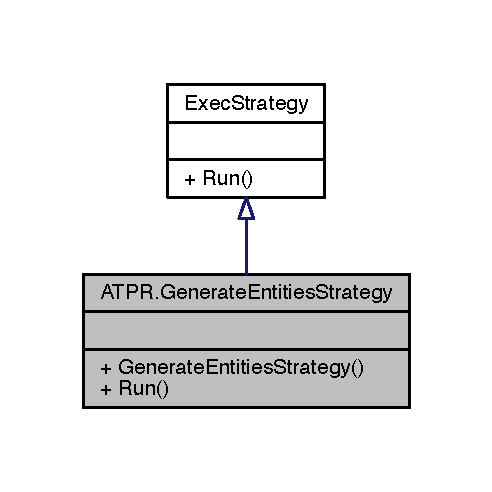
\includegraphics[width=236pt]{de/d9b/class_a_t_p_r_1_1_generate_entities_strategy__inherit__graph}
\end{center}
\end{figure}


Collaboration diagram for A\+T\+P\+R.\+Generate\+Entities\+Strategy\+:
\nopagebreak
\begin{figure}[H]
\begin{center}
\leavevmode
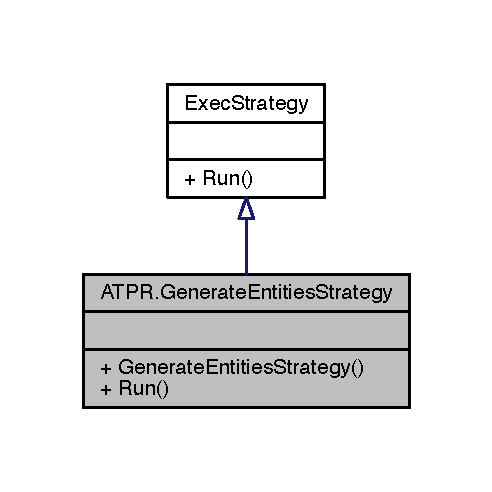
\includegraphics[width=236pt]{d1/d22/class_a_t_p_r_1_1_generate_entities_strategy__coll__graph}
\end{center}
\end{figure}
\subsection*{Public Member Functions}
\begin{DoxyCompactItemize}
\item 
\hyperlink{class_a_t_p_r_1_1_generate_entities_strategy_a9c720ecc2374f2ca6528ccacf422b327}{Generate\+Entities\+Strategy} ()
\begin{DoxyCompactList}\small\item\em Initializes a new instance of the \hyperlink{class_a_t_p_r_1_1_generate_entities_strategy}{A\+T\+P\+R.\+Generate\+Entities\+Strategy} class. \end{DoxyCompactList}\item 
void \hyperlink{class_a_t_p_r_1_1_generate_entities_strategy_a05c83e5d9d7ea2b05f4de5dab1a87f06}{Run} (\hyperlink{class_a_t_p_r_1_1_options}{Options} options)
\begin{DoxyCompactList}\small\item\em Generates an entities X\+ML from N\+ER output. \end{DoxyCompactList}\end{DoxyCompactItemize}


\subsection{Detailed Description}
s\+Strategy class that check generate entities command arguments and execute generate entities. 



\subsection{Constructor \& Destructor Documentation}
\hypertarget{class_a_t_p_r_1_1_generate_entities_strategy_a9c720ecc2374f2ca6528ccacf422b327}{}\label{class_a_t_p_r_1_1_generate_entities_strategy_a9c720ecc2374f2ca6528ccacf422b327} 
\index{A\+T\+P\+R\+::\+Generate\+Entities\+Strategy@{A\+T\+P\+R\+::\+Generate\+Entities\+Strategy}!Generate\+Entities\+Strategy@{Generate\+Entities\+Strategy}}
\index{Generate\+Entities\+Strategy@{Generate\+Entities\+Strategy}!A\+T\+P\+R\+::\+Generate\+Entities\+Strategy@{A\+T\+P\+R\+::\+Generate\+Entities\+Strategy}}
\subsubsection{\texorpdfstring{Generate\+Entities\+Strategy()}{GenerateEntitiesStrategy()}}
{\footnotesize\ttfamily A\+T\+P\+R.\+Generate\+Entities\+Strategy.\+Generate\+Entities\+Strategy (\begin{DoxyParamCaption}{ }\end{DoxyParamCaption})\hspace{0.3cm}{\ttfamily [inline]}}



Initializes a new instance of the \hyperlink{class_a_t_p_r_1_1_generate_entities_strategy}{A\+T\+P\+R.\+Generate\+Entities\+Strategy} class. 



\subsection{Member Function Documentation}
\hypertarget{class_a_t_p_r_1_1_generate_entities_strategy_a05c83e5d9d7ea2b05f4de5dab1a87f06}{}\label{class_a_t_p_r_1_1_generate_entities_strategy_a05c83e5d9d7ea2b05f4de5dab1a87f06} 
\index{A\+T\+P\+R\+::\+Generate\+Entities\+Strategy@{A\+T\+P\+R\+::\+Generate\+Entities\+Strategy}!Run@{Run}}
\index{Run@{Run}!A\+T\+P\+R\+::\+Generate\+Entities\+Strategy@{A\+T\+P\+R\+::\+Generate\+Entities\+Strategy}}
\subsubsection{\texorpdfstring{Run()}{Run()}}
{\footnotesize\ttfamily void A\+T\+P\+R.\+Generate\+Entities\+Strategy.\+Run (\begin{DoxyParamCaption}\item[{\hyperlink{class_a_t_p_r_1_1_options}{Options}}]{options }\end{DoxyParamCaption})\hspace{0.3cm}{\ttfamily [inline]}}



Generates an entities X\+ML from N\+ER output. 


\begin{DoxyParams}{Parameters}
{\em options} & \hyperlink{class_a_t_p_r_1_1_options}{Options}.\\
\hline
\end{DoxyParams}


Implements \hyperlink{interface_a_t_p_r_1_1_exec_strategy}{A\+T\+P\+R.\+Exec\+Strategy}.

Here is the call graph for this function\+:
\nopagebreak
\begin{figure}[H]
\begin{center}
\leavevmode
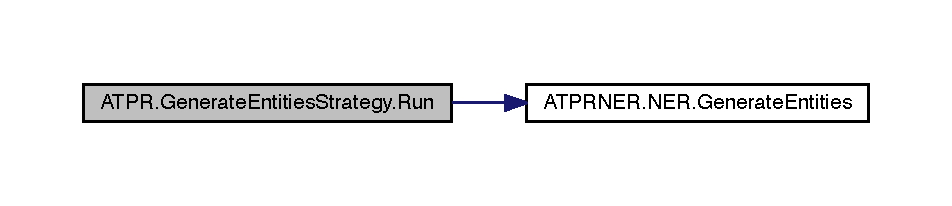
\includegraphics[width=350pt]{de/d99/class_a_t_p_r_1_1_generate_entities_strategy_a05c83e5d9d7ea2b05f4de5dab1a87f06_cgraph}
\end{center}
\end{figure}


The documentation for this class was generated from the following file\+:\begin{DoxyCompactItemize}
\item 
A\+T\+P\+R/Generate\+Entities\+Strategy.\+cs\end{DoxyCompactItemize}

\hypertarget{class_a_t_p_r_1_1_main_class}{}\section{A\+T\+P\+R.\+Main\+Class Class Reference}
\label{class_a_t_p_r_1_1_main_class}\index{A\+T\+P\+R.\+Main\+Class@{A\+T\+P\+R.\+Main\+Class}}


The documentation for this class was generated from the following file\+:\begin{DoxyCompactItemize}
\item 
A\+T\+P\+R/Program.\+cs\end{DoxyCompactItemize}

\hypertarget{class_a_t_p_r_parser_1_1_main_class}{}\section{A\+T\+P\+R\+Parser.\+Main\+Class Class Reference}
\label{class_a_t_p_r_parser_1_1_main_class}\index{A\+T\+P\+R\+Parser.\+Main\+Class@{A\+T\+P\+R\+Parser.\+Main\+Class}}


Collaboration diagram for A\+T\+P\+R\+Parser.\+Main\+Class\+:
\nopagebreak
\begin{figure}[H]
\begin{center}
\leavevmode
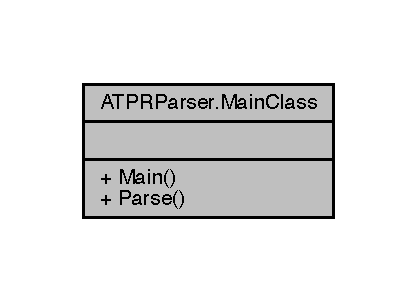
\includegraphics[width=200pt]{de/d7a/class_a_t_p_r_parser_1_1_main_class__coll__graph}
\end{center}
\end{figure}
\subsection*{Static Public Member Functions}
\begin{DoxyCompactItemize}
\item 
static void \hyperlink{class_a_t_p_r_parser_1_1_main_class_ade65079470bbddf6148ad515cb75e389}{Main} (string\mbox{[}$\,$\mbox{]} args)
\begin{DoxyCompactList}\small\item\em The entry point of the program, where the program control starts and ends. \end{DoxyCompactList}\item 
static void \hyperlink{class_a_t_p_r_parser_1_1_main_class_af792fa155ddd2ec39f158270b2dae720}{Parse} (string sentence)
\begin{DoxyCompactList}\small\item\em Parse the specified sentence. \end{DoxyCompactList}\end{DoxyCompactItemize}


\subsection{Member Function Documentation}
\hypertarget{class_a_t_p_r_parser_1_1_main_class_ade65079470bbddf6148ad515cb75e389}{}\label{class_a_t_p_r_parser_1_1_main_class_ade65079470bbddf6148ad515cb75e389} 
\index{A\+T\+P\+R\+Parser\+::\+Main\+Class@{A\+T\+P\+R\+Parser\+::\+Main\+Class}!Main@{Main}}
\index{Main@{Main}!A\+T\+P\+R\+Parser\+::\+Main\+Class@{A\+T\+P\+R\+Parser\+::\+Main\+Class}}
\subsubsection{\texorpdfstring{Main()}{Main()}}
{\footnotesize\ttfamily static void A\+T\+P\+R\+Parser.\+Main\+Class.\+Main (\begin{DoxyParamCaption}\item[{string \mbox{[}$\,$\mbox{]}}]{args }\end{DoxyParamCaption})\hspace{0.3cm}{\ttfamily [inline]}, {\ttfamily [static]}}



The entry point of the program, where the program control starts and ends. 


\begin{DoxyParams}{Parameters}
{\em args} & The command-\/line arguments.\\
\hline
\end{DoxyParams}
\hypertarget{class_a_t_p_r_parser_1_1_main_class_af792fa155ddd2ec39f158270b2dae720}{}\label{class_a_t_p_r_parser_1_1_main_class_af792fa155ddd2ec39f158270b2dae720} 
\index{A\+T\+P\+R\+Parser\+::\+Main\+Class@{A\+T\+P\+R\+Parser\+::\+Main\+Class}!Parse@{Parse}}
\index{Parse@{Parse}!A\+T\+P\+R\+Parser\+::\+Main\+Class@{A\+T\+P\+R\+Parser\+::\+Main\+Class}}
\subsubsection{\texorpdfstring{Parse()}{Parse()}}
{\footnotesize\ttfamily static void A\+T\+P\+R\+Parser.\+Main\+Class.\+Parse (\begin{DoxyParamCaption}\item[{string}]{sentence }\end{DoxyParamCaption})\hspace{0.3cm}{\ttfamily [inline]}, {\ttfamily [static]}}



Parse the specified sentence. 


\begin{DoxyParams}{Parameters}
{\em Sentence} & Sentence to parse\\
\hline
\end{DoxyParams}


The documentation for this class was generated from the following file\+:\begin{DoxyCompactItemize}
\item 
A\+T\+P\+R\+P\+A\+R\+S\+E\+R/Program.\+cs\end{DoxyCompactItemize}

\hypertarget{class_a_t_p_r_n_e_r_1_1_matched_entity}{}\section{A\+T\+P\+R\+N\+E\+R.\+Matched\+Entity Class Reference}
\label{class_a_t_p_r_n_e_r_1_1_matched_entity}\index{A\+T\+P\+R\+N\+E\+R.\+Matched\+Entity@{A\+T\+P\+R\+N\+E\+R.\+Matched\+Entity}}


Represents the matched entitiy with the information needed.  




Collaboration diagram for A\+T\+P\+R\+N\+E\+R.\+Matched\+Entity\+:\nopagebreak
\begin{figure}[H]
\begin{center}
\leavevmode
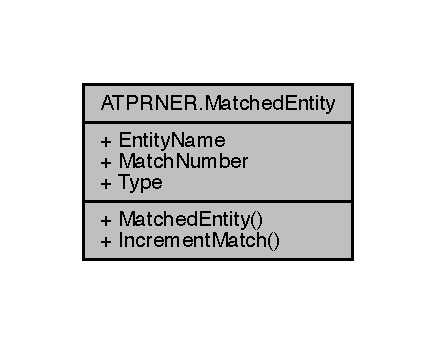
\includegraphics[width=209pt]{d6/dd7/class_a_t_p_r_n_e_r_1_1_matched_entity__coll__graph}
\end{center}
\end{figure}
\subsection*{Public Member Functions}
\begin{DoxyCompactItemize}
\item 
\hyperlink{class_a_t_p_r_n_e_r_1_1_matched_entity_a5737ccd3008395ca92559e0b1b1f3e73}{Matched\+Entity} (String entity\+Name, String type)
\begin{DoxyCompactList}\small\item\em Initializes a new instance of the \hyperlink{class_a_t_p_r_n_e_r_1_1_matched_entity}{A\+T\+P\+R\+N\+E\+R.\+Matched\+Entity} class. \end{DoxyCompactList}\item 
void \hyperlink{class_a_t_p_r_n_e_r_1_1_matched_entity_ae6fa09ea42c0787d4279ceb5076c5f14}{Increment\+Match} ()
\begin{DoxyCompactList}\small\item\em Increments the match number one unity. \end{DoxyCompactList}\end{DoxyCompactItemize}
\subsection*{Properties}
\begin{DoxyCompactItemize}
\item 
String \hyperlink{class_a_t_p_r_n_e_r_1_1_matched_entity_a42a05257a07b5d089ac070b1d9e5461a}{Entity\+Name}\hspace{0.3cm}{\ttfamily  \mbox{[}get, set\mbox{]}}
\begin{DoxyCompactList}\small\item\em Gets or sets the name of the entity. \end{DoxyCompactList}\item 
int \hyperlink{class_a_t_p_r_n_e_r_1_1_matched_entity_ad6ca936e2b54158984f7d7d3753d1490}{Match\+Number}\hspace{0.3cm}{\ttfamily  \mbox{[}get, set\mbox{]}}
\begin{DoxyCompactList}\small\item\em Gets or sets the match number. \end{DoxyCompactList}\item 
String \hyperlink{class_a_t_p_r_n_e_r_1_1_matched_entity_af7d651ec944931f14c26eedffc4150de}{Type}\hspace{0.3cm}{\ttfamily  \mbox{[}get, set\mbox{]}}
\begin{DoxyCompactList}\small\item\em Gets or sets the type. \end{DoxyCompactList}\end{DoxyCompactItemize}


\subsection{Detailed Description}
Represents the matched entitiy with the information needed. 



\subsection{Constructor \& Destructor Documentation}
\hypertarget{class_a_t_p_r_n_e_r_1_1_matched_entity_a5737ccd3008395ca92559e0b1b1f3e73}{}\label{class_a_t_p_r_n_e_r_1_1_matched_entity_a5737ccd3008395ca92559e0b1b1f3e73} 
\index{A\+T\+P\+R\+N\+E\+R\+::\+Matched\+Entity@{A\+T\+P\+R\+N\+E\+R\+::\+Matched\+Entity}!Matched\+Entity@{Matched\+Entity}}
\index{Matched\+Entity@{Matched\+Entity}!A\+T\+P\+R\+N\+E\+R\+::\+Matched\+Entity@{A\+T\+P\+R\+N\+E\+R\+::\+Matched\+Entity}}
\subsubsection{\texorpdfstring{Matched\+Entity()}{MatchedEntity()}}
{\footnotesize\ttfamily A\+T\+P\+R\+N\+E\+R.\+Matched\+Entity.\+Matched\+Entity (\begin{DoxyParamCaption}\item[{String}]{entity\+Name,  }\item[{String}]{type }\end{DoxyParamCaption})\hspace{0.3cm}{\ttfamily [inline]}}



Initializes a new instance of the \hyperlink{class_a_t_p_r_n_e_r_1_1_matched_entity}{A\+T\+P\+R\+N\+E\+R.\+Matched\+Entity} class. 


\begin{DoxyParams}{Parameters}
{\em entity\+Name} & Entity name.\\
\hline
\end{DoxyParams}


\subsection{Member Function Documentation}
\hypertarget{class_a_t_p_r_n_e_r_1_1_matched_entity_ae6fa09ea42c0787d4279ceb5076c5f14}{}\label{class_a_t_p_r_n_e_r_1_1_matched_entity_ae6fa09ea42c0787d4279ceb5076c5f14} 
\index{A\+T\+P\+R\+N\+E\+R\+::\+Matched\+Entity@{A\+T\+P\+R\+N\+E\+R\+::\+Matched\+Entity}!Increment\+Match@{Increment\+Match}}
\index{Increment\+Match@{Increment\+Match}!A\+T\+P\+R\+N\+E\+R\+::\+Matched\+Entity@{A\+T\+P\+R\+N\+E\+R\+::\+Matched\+Entity}}
\subsubsection{\texorpdfstring{Increment\+Match()}{IncrementMatch()}}
{\footnotesize\ttfamily void A\+T\+P\+R\+N\+E\+R.\+Matched\+Entity.\+Increment\+Match (\begin{DoxyParamCaption}{ }\end{DoxyParamCaption})\hspace{0.3cm}{\ttfamily [inline]}}



Increments the match number one unity. 



\subsection{Property Documentation}
\hypertarget{class_a_t_p_r_n_e_r_1_1_matched_entity_a42a05257a07b5d089ac070b1d9e5461a}{}\label{class_a_t_p_r_n_e_r_1_1_matched_entity_a42a05257a07b5d089ac070b1d9e5461a} 
\index{A\+T\+P\+R\+N\+E\+R\+::\+Matched\+Entity@{A\+T\+P\+R\+N\+E\+R\+::\+Matched\+Entity}!Entity\+Name@{Entity\+Name}}
\index{Entity\+Name@{Entity\+Name}!A\+T\+P\+R\+N\+E\+R\+::\+Matched\+Entity@{A\+T\+P\+R\+N\+E\+R\+::\+Matched\+Entity}}
\subsubsection{\texorpdfstring{Entity\+Name}{EntityName}}
{\footnotesize\ttfamily String A\+T\+P\+R\+N\+E\+R.\+Matched\+Entity.\+Entity\+Name\hspace{0.3cm}{\ttfamily [get]}, {\ttfamily [set]}}



Gets or sets the name of the entity. 

The name of the entity.\hypertarget{class_a_t_p_r_n_e_r_1_1_matched_entity_ad6ca936e2b54158984f7d7d3753d1490}{}\label{class_a_t_p_r_n_e_r_1_1_matched_entity_ad6ca936e2b54158984f7d7d3753d1490} 
\index{A\+T\+P\+R\+N\+E\+R\+::\+Matched\+Entity@{A\+T\+P\+R\+N\+E\+R\+::\+Matched\+Entity}!Match\+Number@{Match\+Number}}
\index{Match\+Number@{Match\+Number}!A\+T\+P\+R\+N\+E\+R\+::\+Matched\+Entity@{A\+T\+P\+R\+N\+E\+R\+::\+Matched\+Entity}}
\subsubsection{\texorpdfstring{Match\+Number}{MatchNumber}}
{\footnotesize\ttfamily int A\+T\+P\+R\+N\+E\+R.\+Matched\+Entity.\+Match\+Number\hspace{0.3cm}{\ttfamily [get]}, {\ttfamily [set]}}



Gets or sets the match number. 

The match number.\hypertarget{class_a_t_p_r_n_e_r_1_1_matched_entity_af7d651ec944931f14c26eedffc4150de}{}\label{class_a_t_p_r_n_e_r_1_1_matched_entity_af7d651ec944931f14c26eedffc4150de} 
\index{A\+T\+P\+R\+N\+E\+R\+::\+Matched\+Entity@{A\+T\+P\+R\+N\+E\+R\+::\+Matched\+Entity}!Type@{Type}}
\index{Type@{Type}!A\+T\+P\+R\+N\+E\+R\+::\+Matched\+Entity@{A\+T\+P\+R\+N\+E\+R\+::\+Matched\+Entity}}
\subsubsection{\texorpdfstring{Type}{Type}}
{\footnotesize\ttfamily String A\+T\+P\+R\+N\+E\+R.\+Matched\+Entity.\+Type\hspace{0.3cm}{\ttfamily [get]}, {\ttfamily [set]}}



Gets or sets the type. 

The type.

The documentation for this class was generated from the following file\+:\begin{DoxyCompactItemize}
\item 
A\+T\+P\+R\+N\+E\+R/Matched\+Entity.\+cs\end{DoxyCompactItemize}

\hypertarget{class_a_t_p_r_1_1_match_entities_strategy}{}\section{A\+T\+P\+R.\+Match\+Entities\+Strategy Class Reference}
\label{class_a_t_p_r_1_1_match_entities_strategy}\index{A\+T\+P\+R.\+Match\+Entities\+Strategy@{A\+T\+P\+R.\+Match\+Entities\+Strategy}}


Strategy class that generates the matches between textentities and dictionary entities.  




Inheritance diagram for A\+T\+P\+R.\+Match\+Entities\+Strategy\+:
\nopagebreak
\begin{figure}[H]
\begin{center}
\leavevmode
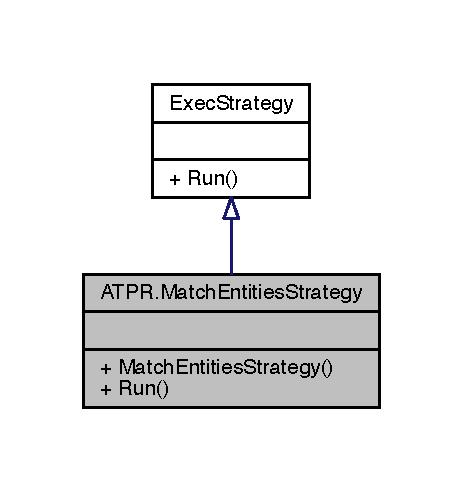
\includegraphics[width=222pt]{d6/d4b/class_a_t_p_r_1_1_match_entities_strategy__inherit__graph}
\end{center}
\end{figure}


Collaboration diagram for A\+T\+P\+R.\+Match\+Entities\+Strategy\+:
\nopagebreak
\begin{figure}[H]
\begin{center}
\leavevmode
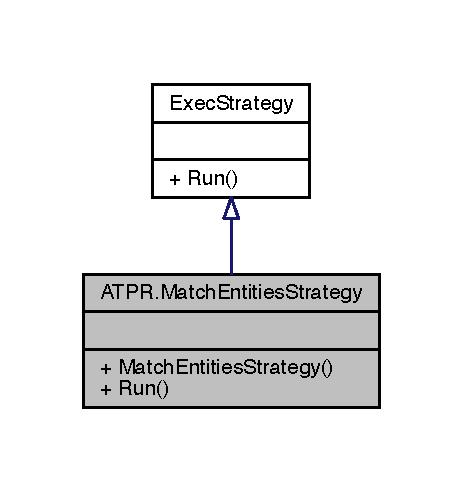
\includegraphics[width=222pt]{d9/dfa/class_a_t_p_r_1_1_match_entities_strategy__coll__graph}
\end{center}
\end{figure}
\subsection*{Public Member Functions}
\begin{DoxyCompactItemize}
\item 
\hyperlink{class_a_t_p_r_1_1_match_entities_strategy_a21587dd85c37c7796b4cd4e48bc85459}{Match\+Entities\+Strategy} ()
\begin{DoxyCompactList}\small\item\em Initializes a new instance of the \hyperlink{class_a_t_p_r_1_1_match_entities_strategy}{A\+T\+P\+R.\+Match\+Entities\+Strategy} class. \end{DoxyCompactList}\item 
void \hyperlink{class_a_t_p_r_1_1_match_entities_strategy_a7494fa761f1e14c463b4c6e5614ae1c4}{Run} (\hyperlink{class_a_t_p_r_1_1_options}{Options} options)
\begin{DoxyCompactList}\small\item\em Generates the match between textentities and dictionary entities. \end{DoxyCompactList}\end{DoxyCompactItemize}


\subsection{Detailed Description}
Strategy class that generates the matches between textentities and dictionary entities. 



\subsection{Constructor \& Destructor Documentation}
\hypertarget{class_a_t_p_r_1_1_match_entities_strategy_a21587dd85c37c7796b4cd4e48bc85459}{}\label{class_a_t_p_r_1_1_match_entities_strategy_a21587dd85c37c7796b4cd4e48bc85459} 
\index{A\+T\+P\+R\+::\+Match\+Entities\+Strategy@{A\+T\+P\+R\+::\+Match\+Entities\+Strategy}!Match\+Entities\+Strategy@{Match\+Entities\+Strategy}}
\index{Match\+Entities\+Strategy@{Match\+Entities\+Strategy}!A\+T\+P\+R\+::\+Match\+Entities\+Strategy@{A\+T\+P\+R\+::\+Match\+Entities\+Strategy}}
\subsubsection{\texorpdfstring{Match\+Entities\+Strategy()}{MatchEntitiesStrategy()}}
{\footnotesize\ttfamily A\+T\+P\+R.\+Match\+Entities\+Strategy.\+Match\+Entities\+Strategy (\begin{DoxyParamCaption}{ }\end{DoxyParamCaption})\hspace{0.3cm}{\ttfamily [inline]}}



Initializes a new instance of the \hyperlink{class_a_t_p_r_1_1_match_entities_strategy}{A\+T\+P\+R.\+Match\+Entities\+Strategy} class. 



\subsection{Member Function Documentation}
\hypertarget{class_a_t_p_r_1_1_match_entities_strategy_a7494fa761f1e14c463b4c6e5614ae1c4}{}\label{class_a_t_p_r_1_1_match_entities_strategy_a7494fa761f1e14c463b4c6e5614ae1c4} 
\index{A\+T\+P\+R\+::\+Match\+Entities\+Strategy@{A\+T\+P\+R\+::\+Match\+Entities\+Strategy}!Run@{Run}}
\index{Run@{Run}!A\+T\+P\+R\+::\+Match\+Entities\+Strategy@{A\+T\+P\+R\+::\+Match\+Entities\+Strategy}}
\subsubsection{\texorpdfstring{Run()}{Run()}}
{\footnotesize\ttfamily void A\+T\+P\+R.\+Match\+Entities\+Strategy.\+Run (\begin{DoxyParamCaption}\item[{\hyperlink{class_a_t_p_r_1_1_options}{Options}}]{options }\end{DoxyParamCaption})\hspace{0.3cm}{\ttfamily [inline]}}



Generates the match between textentities and dictionary entities. 


\begin{DoxyParams}{Parameters}
{\em options} & \hyperlink{class_a_t_p_r_1_1_options}{Options}.\\
\hline
\end{DoxyParams}


Implements \hyperlink{interface_a_t_p_r_1_1_exec_strategy}{A\+T\+P\+R.\+Exec\+Strategy}.

Here is the call graph for this function\+:
\nopagebreak
\begin{figure}[H]
\begin{center}
\leavevmode
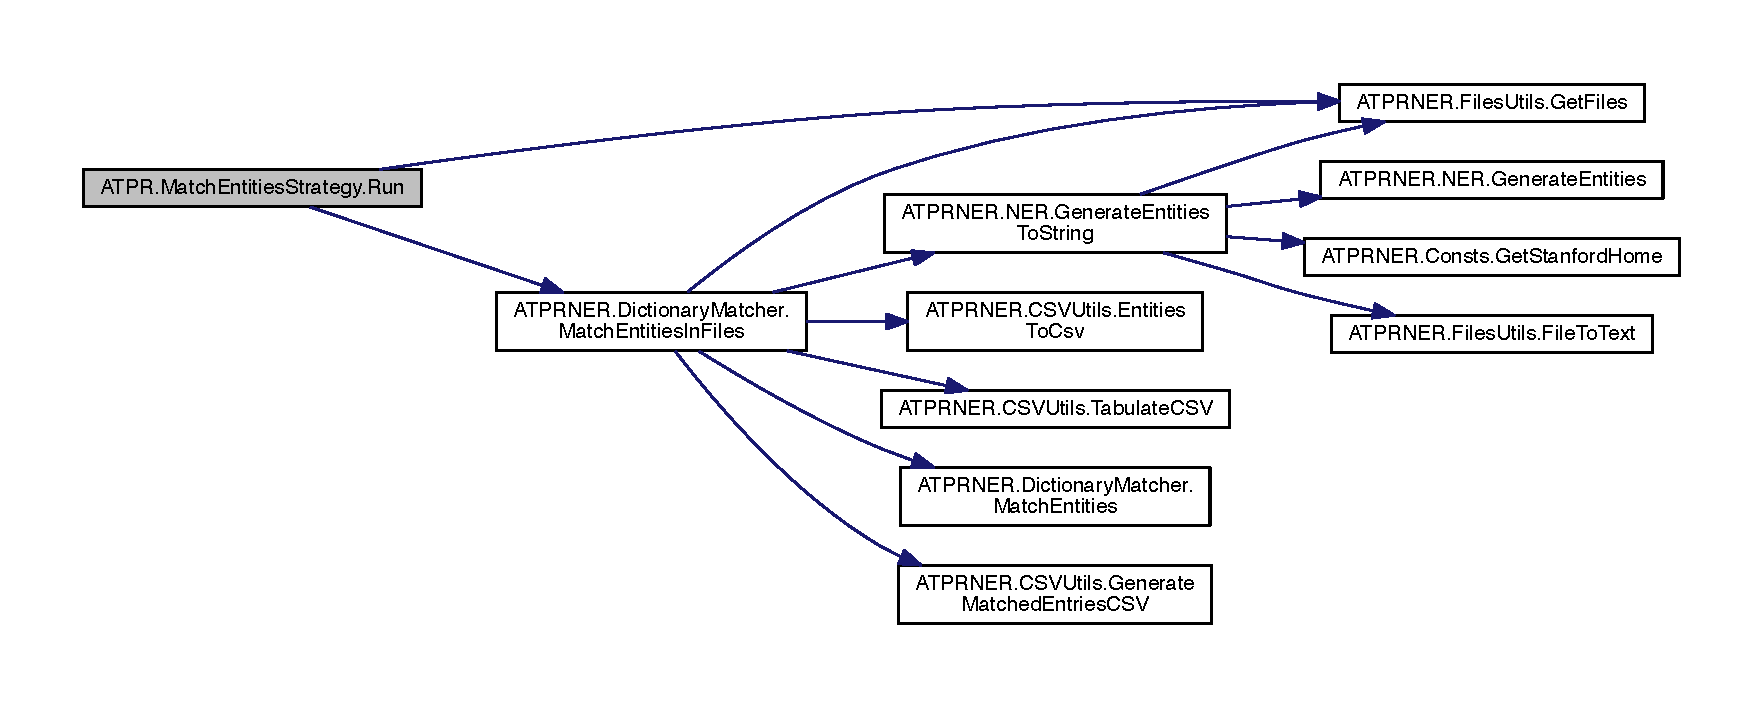
\includegraphics[width=350pt]{df/db7/class_a_t_p_r_1_1_match_entities_strategy_a7494fa761f1e14c463b4c6e5614ae1c4_cgraph}
\end{center}
\end{figure}


The documentation for this class was generated from the following file\+:\begin{DoxyCompactItemize}
\item 
A\+T\+P\+R/Match\+Entities\+Strategy.\+cs\end{DoxyCompactItemize}

\hypertarget{class_a_t_p_r_n_e_r_1_1_n_e_r}{}\section{A\+T\+P\+R\+N\+E\+R.\+N\+ER Class Reference}
\label{class_a_t_p_r_n_e_r_1_1_n_e_r}\index{A\+T\+P\+R\+N\+E\+R.\+N\+ER@{A\+T\+P\+R\+N\+E\+R.\+N\+ER}}


Collaboration diagram for A\+T\+P\+R\+N\+E\+R.\+N\+ER\+:
\nopagebreak
\begin{figure}[H]
\begin{center}
\leavevmode
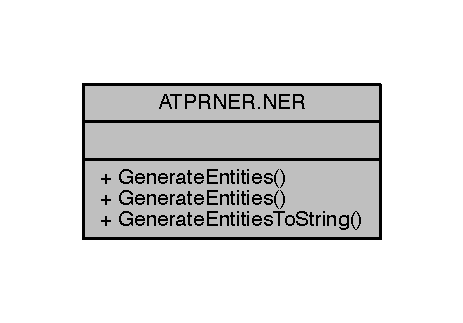
\includegraphics[width=222pt]{d2/d33/class_a_t_p_r_n_e_r_1_1_n_e_r__coll__graph}
\end{center}
\end{figure}
\subsection*{Static Public Member Functions}
\begin{DoxyCompactItemize}
\item 
static void \hyperlink{class_a_t_p_r_n_e_r_1_1_n_e_r_ac52e8765543f6342e2fb0fd4283f10d7}{Generate\+Entities} (string input\+Path, string output\+Path)
\begin{DoxyCompactList}\small\item\em Generates the dict from the documents in input\+Path and send output to output file in output\+Path \end{DoxyCompactList}\item 
static void \hyperlink{class_a_t_p_r_n_e_r_1_1_n_e_r_afbf080a32a868531adb8c7f4ec5f8035}{Generate\+Entities} (string input\+Path)
\begin{DoxyCompactList}\small\item\em Generates the dict from the documents in input\+Path and send output to stdout \end{DoxyCompactList}\item 
static string \hyperlink{class_a_t_p_r_n_e_r_1_1_n_e_r_a8480137d05620d726021a2f4ae818869}{Generate\+Entities\+To\+String} (string input\+Path)
\begin{DoxyCompactList}\small\item\em Generates the dict from the documents in input\+Path and send output to a string. \end{DoxyCompactList}\end{DoxyCompactItemize}


\subsection{Member Function Documentation}
\hypertarget{class_a_t_p_r_n_e_r_1_1_n_e_r_ac52e8765543f6342e2fb0fd4283f10d7}{}\label{class_a_t_p_r_n_e_r_1_1_n_e_r_ac52e8765543f6342e2fb0fd4283f10d7} 
\index{A\+T\+P\+R\+N\+E\+R\+::\+N\+ER@{A\+T\+P\+R\+N\+E\+R\+::\+N\+ER}!Generate\+Entities@{Generate\+Entities}}
\index{Generate\+Entities@{Generate\+Entities}!A\+T\+P\+R\+N\+E\+R\+::\+N\+ER@{A\+T\+P\+R\+N\+E\+R\+::\+N\+ER}}
\subsubsection{\texorpdfstring{Generate\+Entities()}{GenerateEntities()}\hspace{0.1cm}{\footnotesize\ttfamily [1/2]}}
{\footnotesize\ttfamily static void A\+T\+P\+R\+N\+E\+R.\+N\+E\+R.\+Generate\+Entities (\begin{DoxyParamCaption}\item[{string}]{input\+Path,  }\item[{string}]{output\+Path }\end{DoxyParamCaption})\hspace{0.3cm}{\ttfamily [inline]}, {\ttfamily [static]}}



Generates the dict from the documents in input\+Path and send output to output file in output\+Path 


\begin{DoxyParams}{Parameters}
{\em input\+Path} & Input path.\\
\hline
{\em output\+Path} & Output path.\\
\hline
\end{DoxyParams}
Here is the caller graph for this function\+:
\nopagebreak
\begin{figure}[H]
\begin{center}
\leavevmode
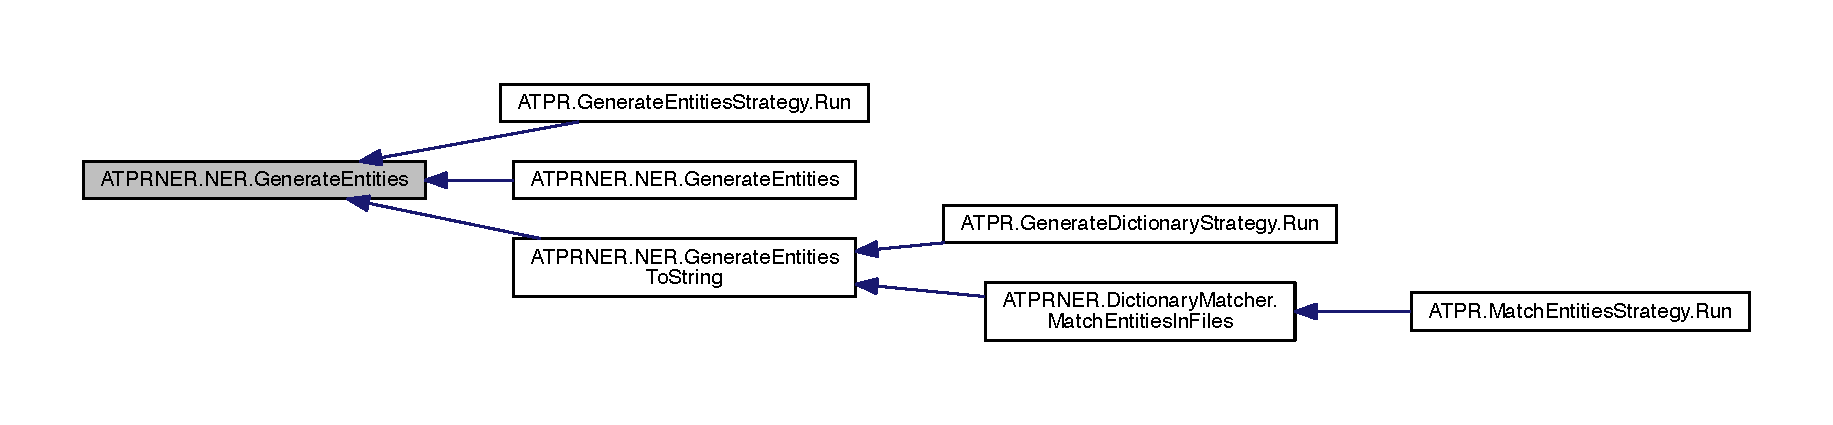
\includegraphics[width=350pt]{d5/dec/class_a_t_p_r_n_e_r_1_1_n_e_r_ac52e8765543f6342e2fb0fd4283f10d7_icgraph}
\end{center}
\end{figure}
\hypertarget{class_a_t_p_r_n_e_r_1_1_n_e_r_afbf080a32a868531adb8c7f4ec5f8035}{}\label{class_a_t_p_r_n_e_r_1_1_n_e_r_afbf080a32a868531adb8c7f4ec5f8035} 
\index{A\+T\+P\+R\+N\+E\+R\+::\+N\+ER@{A\+T\+P\+R\+N\+E\+R\+::\+N\+ER}!Generate\+Entities@{Generate\+Entities}}
\index{Generate\+Entities@{Generate\+Entities}!A\+T\+P\+R\+N\+E\+R\+::\+N\+ER@{A\+T\+P\+R\+N\+E\+R\+::\+N\+ER}}
\subsubsection{\texorpdfstring{Generate\+Entities()}{GenerateEntities()}\hspace{0.1cm}{\footnotesize\ttfamily [2/2]}}
{\footnotesize\ttfamily static void A\+T\+P\+R\+N\+E\+R.\+N\+E\+R.\+Generate\+Entities (\begin{DoxyParamCaption}\item[{string}]{input\+Path }\end{DoxyParamCaption})\hspace{0.3cm}{\ttfamily [inline]}, {\ttfamily [static]}}



Generates the dict from the documents in input\+Path and send output to stdout 


\begin{DoxyParams}{Parameters}
{\em input\+Path} & Input path.\\
\hline
\end{DoxyParams}
Here is the call graph for this function\+:
\nopagebreak
\begin{figure}[H]
\begin{center}
\leavevmode
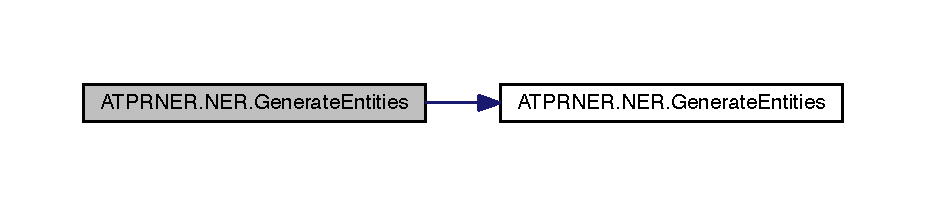
\includegraphics[width=350pt]{d5/dec/class_a_t_p_r_n_e_r_1_1_n_e_r_afbf080a32a868531adb8c7f4ec5f8035_cgraph}
\end{center}
\end{figure}
\hypertarget{class_a_t_p_r_n_e_r_1_1_n_e_r_a8480137d05620d726021a2f4ae818869}{}\label{class_a_t_p_r_n_e_r_1_1_n_e_r_a8480137d05620d726021a2f4ae818869} 
\index{A\+T\+P\+R\+N\+E\+R\+::\+N\+ER@{A\+T\+P\+R\+N\+E\+R\+::\+N\+ER}!Generate\+Entities\+To\+String@{Generate\+Entities\+To\+String}}
\index{Generate\+Entities\+To\+String@{Generate\+Entities\+To\+String}!A\+T\+P\+R\+N\+E\+R\+::\+N\+ER@{A\+T\+P\+R\+N\+E\+R\+::\+N\+ER}}
\subsubsection{\texorpdfstring{Generate\+Entities\+To\+String()}{GenerateEntitiesToString()}}
{\footnotesize\ttfamily static string A\+T\+P\+R\+N\+E\+R.\+N\+E\+R.\+Generate\+Entities\+To\+String (\begin{DoxyParamCaption}\item[{string}]{input\+Path }\end{DoxyParamCaption})\hspace{0.3cm}{\ttfamily [inline]}, {\ttfamily [static]}}



Generates the dict from the documents in input\+Path and send output to a string. 

\begin{DoxyReturn}{Returns}
The entities xml.
\end{DoxyReturn}

\begin{DoxyParams}{Parameters}
{\em input\+Path} & Input path.\\
\hline
\end{DoxyParams}
Here is the call graph for this function\+:
\nopagebreak
\begin{figure}[H]
\begin{center}
\leavevmode
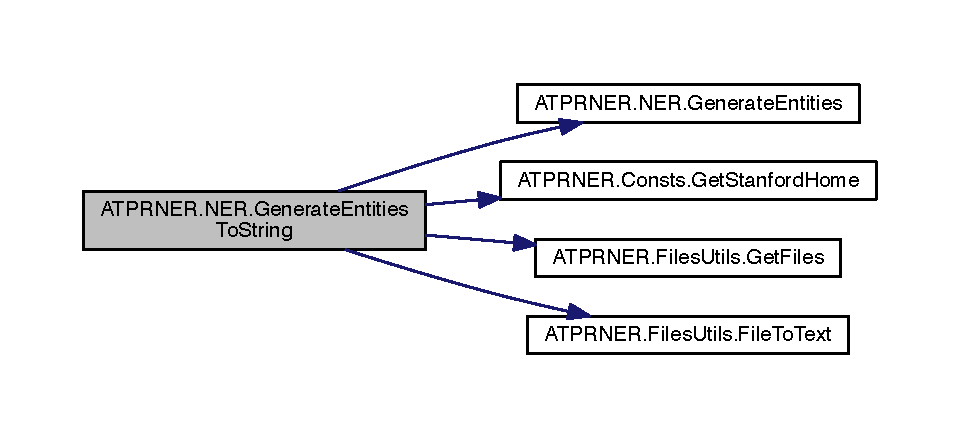
\includegraphics[width=350pt]{d5/dec/class_a_t_p_r_n_e_r_1_1_n_e_r_a8480137d05620d726021a2f4ae818869_cgraph}
\end{center}
\end{figure}
Here is the caller graph for this function\+:
\nopagebreak
\begin{figure}[H]
\begin{center}
\leavevmode
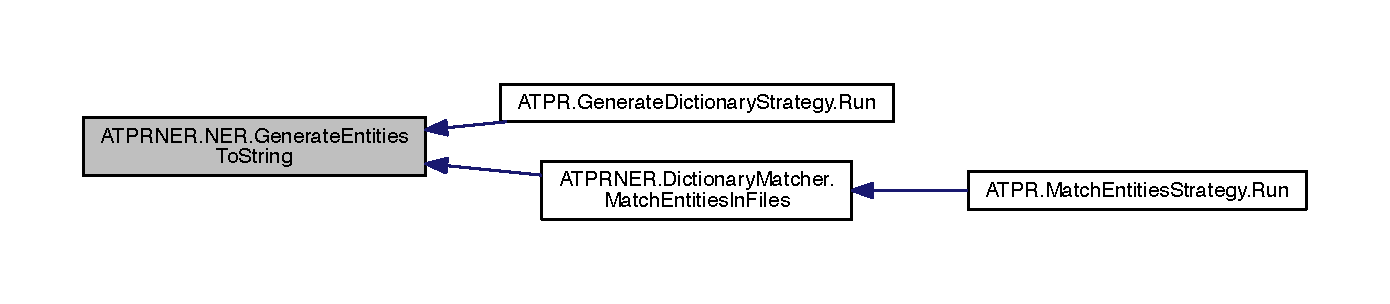
\includegraphics[width=350pt]{d5/dec/class_a_t_p_r_n_e_r_1_1_n_e_r_a8480137d05620d726021a2f4ae818869_icgraph}
\end{center}
\end{figure}


The documentation for this class was generated from the following file\+:\begin{DoxyCompactItemize}
\item 
A\+T\+P\+R\+N\+E\+R/N\+E\+R.\+cs\end{DoxyCompactItemize}

\hypertarget{class_a_t_p_r_1_1_options}{}\section{A\+T\+P\+R.\+Options Class Reference}
\label{class_a_t_p_r_1_1_options}\index{A\+T\+P\+R.\+Options@{A\+T\+P\+R.\+Options}}


Argument parse options.  




Collaboration diagram for A\+T\+P\+R.\+Options\+:
\nopagebreak
\begin{figure}[H]
\begin{center}
\leavevmode
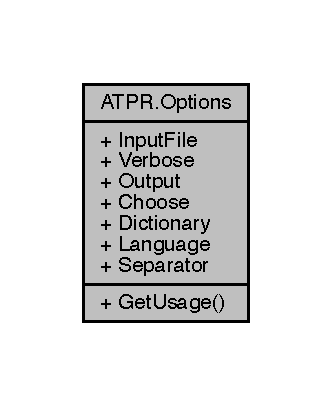
\includegraphics[width=159pt]{d4/dc3/class_a_t_p_r_1_1_options__coll__graph}
\end{center}
\end{figure}
\subsection*{Public Member Functions}
\begin{DoxyCompactItemize}
\item 
\hypertarget{class_a_t_p_r_1_1_options_a92883d4a7564f235412e41e6724c32b2}{}\label{class_a_t_p_r_1_1_options_a92883d4a7564f235412e41e6724c32b2} 
string {\bfseries Get\+Usage} ()
\end{DoxyCompactItemize}
\subsection*{Properties}
\begin{DoxyCompactItemize}
\item 
\hypertarget{class_a_t_p_r_1_1_options_ac0a2d51d6f7ef81700651d3951f51e4f}{}\label{class_a_t_p_r_1_1_options_ac0a2d51d6f7ef81700651d3951f51e4f} 
string {\bfseries Input\+File}\hspace{0.3cm}{\ttfamily  \mbox{[}get, set\mbox{]}}
\item 
\hypertarget{class_a_t_p_r_1_1_options_a8cb44ee6dbab360a3d9412626c2fa2d9}{}\label{class_a_t_p_r_1_1_options_a8cb44ee6dbab360a3d9412626c2fa2d9} 
bool {\bfseries Verbose}\hspace{0.3cm}{\ttfamily  \mbox{[}get, set\mbox{]}}
\item 
\hypertarget{class_a_t_p_r_1_1_options_a933d1d83e25d63f9b006c48efe3b4fd1}{}\label{class_a_t_p_r_1_1_options_a933d1d83e25d63f9b006c48efe3b4fd1} 
string {\bfseries Output}\hspace{0.3cm}{\ttfamily  \mbox{[}get, set\mbox{]}}
\item 
\hypertarget{class_a_t_p_r_1_1_options_a2b57c8aeea07cb4359ca235c24cd6cfe}{}\label{class_a_t_p_r_1_1_options_a2b57c8aeea07cb4359ca235c24cd6cfe} 
string {\bfseries Choose}\hspace{0.3cm}{\ttfamily  \mbox{[}get, set\mbox{]}}
\item 
\hypertarget{class_a_t_p_r_1_1_options_a5187c31694e58eb5cd7464b3c1f5eacc}{}\label{class_a_t_p_r_1_1_options_a5187c31694e58eb5cd7464b3c1f5eacc} 
string {\bfseries Dictionary}\hspace{0.3cm}{\ttfamily  \mbox{[}get, set\mbox{]}}
\item 
\hypertarget{class_a_t_p_r_1_1_options_af1d36310babdada573488c4795ee9a92}{}\label{class_a_t_p_r_1_1_options_af1d36310babdada573488c4795ee9a92} 
string {\bfseries Language}\hspace{0.3cm}{\ttfamily  \mbox{[}get, set\mbox{]}}
\item 
\hypertarget{class_a_t_p_r_1_1_options_ab40c002e4eeede247c68606cb3481a0f}{}\label{class_a_t_p_r_1_1_options_ab40c002e4eeede247c68606cb3481a0f} 
char {\bfseries Separator}\hspace{0.3cm}{\ttfamily  \mbox{[}get, set\mbox{]}}
\end{DoxyCompactItemize}


\subsection{Detailed Description}
Argument parse options. 



The documentation for this class was generated from the following file\+:\begin{DoxyCompactItemize}
\item 
A\+T\+P\+R/Options.\+cs\end{DoxyCompactItemize}

\hypertarget{class_a_t_p_r_1_1_parse_strategy}{}\section{A\+T\+P\+R.\+Parse\+Strategy Class Reference}
\label{class_a_t_p_r_1_1_parse_strategy}\index{A\+T\+P\+R.\+Parse\+Strategy@{A\+T\+P\+R.\+Parse\+Strategy}}


Strategy class that generate the syntax analisis of the documents using the entities of the matching process result.  




Inheritance diagram for A\+T\+P\+R.\+Parse\+Strategy\+:
\nopagebreak
\begin{figure}[H]
\begin{center}
\leavevmode
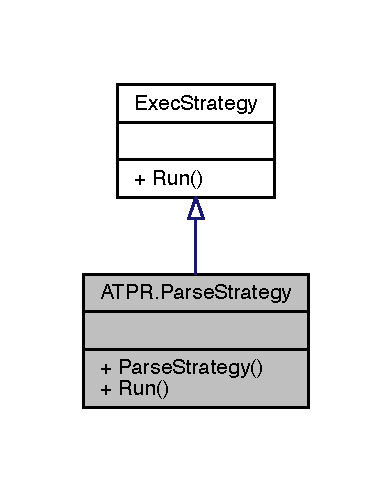
\includegraphics[width=188pt]{d0/d36/class_a_t_p_r_1_1_parse_strategy__inherit__graph}
\end{center}
\end{figure}


Collaboration diagram for A\+T\+P\+R.\+Parse\+Strategy\+:
\nopagebreak
\begin{figure}[H]
\begin{center}
\leavevmode
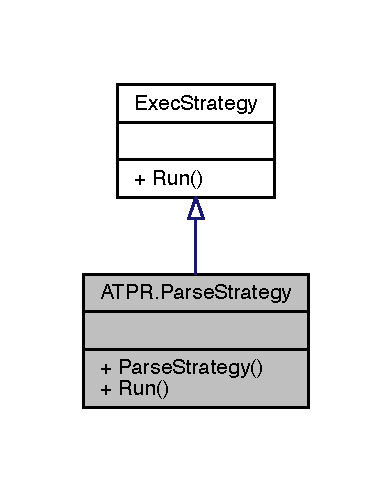
\includegraphics[width=188pt]{d8/d18/class_a_t_p_r_1_1_parse_strategy__coll__graph}
\end{center}
\end{figure}
\subsection*{Public Member Functions}
\begin{DoxyCompactItemize}
\item 
\hyperlink{class_a_t_p_r_1_1_parse_strategy_a9f3b68bd95185518be25cc33d50c8c67}{Parse\+Strategy} ()
\begin{DoxyCompactList}\small\item\em Initializes a new instance of the \hyperlink{class_a_t_p_r_1_1_parse_strategy}{A\+T\+P\+R.\+Parse\+Strategy} class. \end{DoxyCompactList}\item 
void \hyperlink{class_a_t_p_r_1_1_parse_strategy_ae5b4ddf4a1578070dfaa1c332a118438}{Run} (\hyperlink{class_a_t_p_r_1_1_options}{Options} options)
\begin{DoxyCompactList}\small\item\em Run the specified options. Run all the logic of the command. \end{DoxyCompactList}\end{DoxyCompactItemize}


\subsection{Detailed Description}
Strategy class that generate the syntax analisis of the documents using the entities of the matching process result. 



\subsection{Constructor \& Destructor Documentation}
\hypertarget{class_a_t_p_r_1_1_parse_strategy_a9f3b68bd95185518be25cc33d50c8c67}{}\label{class_a_t_p_r_1_1_parse_strategy_a9f3b68bd95185518be25cc33d50c8c67} 
\index{A\+T\+P\+R\+::\+Parse\+Strategy@{A\+T\+P\+R\+::\+Parse\+Strategy}!Parse\+Strategy@{Parse\+Strategy}}
\index{Parse\+Strategy@{Parse\+Strategy}!A\+T\+P\+R\+::\+Parse\+Strategy@{A\+T\+P\+R\+::\+Parse\+Strategy}}
\subsubsection{\texorpdfstring{Parse\+Strategy()}{ParseStrategy()}}
{\footnotesize\ttfamily A\+T\+P\+R.\+Parse\+Strategy.\+Parse\+Strategy (\begin{DoxyParamCaption}{ }\end{DoxyParamCaption})\hspace{0.3cm}{\ttfamily [inline]}}



Initializes a new instance of the \hyperlink{class_a_t_p_r_1_1_parse_strategy}{A\+T\+P\+R.\+Parse\+Strategy} class. 



\subsection{Member Function Documentation}
\hypertarget{class_a_t_p_r_1_1_parse_strategy_ae5b4ddf4a1578070dfaa1c332a118438}{}\label{class_a_t_p_r_1_1_parse_strategy_ae5b4ddf4a1578070dfaa1c332a118438} 
\index{A\+T\+P\+R\+::\+Parse\+Strategy@{A\+T\+P\+R\+::\+Parse\+Strategy}!Run@{Run}}
\index{Run@{Run}!A\+T\+P\+R\+::\+Parse\+Strategy@{A\+T\+P\+R\+::\+Parse\+Strategy}}
\subsubsection{\texorpdfstring{Run()}{Run()}}
{\footnotesize\ttfamily void A\+T\+P\+R.\+Parse\+Strategy.\+Run (\begin{DoxyParamCaption}\item[{\hyperlink{class_a_t_p_r_1_1_options}{Options}}]{options }\end{DoxyParamCaption})\hspace{0.3cm}{\ttfamily [inline]}}



Run the specified options. Run all the logic of the command. 


\begin{DoxyParams}{Parameters}
{\em options} & \hyperlink{class_a_t_p_r_1_1_options}{Options}.\\
\hline
\end{DoxyParams}


Implements \hyperlink{interface_a_t_p_r_1_1_exec_strategy}{A\+T\+P\+R.\+Exec\+Strategy}.



The documentation for this class was generated from the following file\+:\begin{DoxyCompactItemize}
\item 
A\+T\+P\+R/Parse\+Strategy.\+cs\end{DoxyCompactItemize}

%--- End generated contents ---

% Index
\backmatter
\newpage
\phantomsection
\clearemptydoublepage
\addcontentsline{toc}{chapter}{Index}
\printindex

\end{document}
